\documentclass[a4paper]{article}
\usepackage[T1]{fontenc}
\usepackage[latin1]{inputenc}
\usepackage{ngerman}
\usepackage{amsmath}
\usepackage{mathtools}
\usepackage{subfigure}
\usepackage{graphicx}
\usepackage{geometry}
\usepackage{caption}
\usepackage{amsmath}
\usepackage{wrapfig}
\usepackage{listings}
\usepackage{titling}
\usepackage{color}
\usepackage{hyperref}
\usepackage[bottom]{footmisc}
\usepackage[toc,page]{appendix}
\input{kvmacros}	% kv diagram
\usepackage{tikz}
\usepackage{circuitikz} % circuit, logic gate
\usepackage{tikz-timing}
\usepackage{float}			% f�r den text fluss um figures und tables
\usepackage{placeins}
\usepackage{multirow}
\usepackage{todonotes}
\usepackage{wrapfig}
\usepackage{multicol}
\usetikzlibrary{arrows,automata}
\graphicspath{{./pics/}}
\geometry{
	left=25mm,
	top=20mm,
	right=20mm,
	bottom=20mm
}

\lstset{ captionpos=b,
		 rulecolor=\color{black},
		 breaklines=true,
		 frame=single
	   }

\pretitle{%
	\begin{center}
		\LARGE
		{
\includegraphics[width=0.6\textwidth]{logo.png}}\\[\bigskipamount]
	}
	\posttitle{\end{center}}

\title{\textbf{Programmierbare Logik \\ Laborbericht}}
\author{Wintersemester 2018/2019\\\\\\
	Gruppe:		\\\\
	Baga, Oleksandra  (Matr.-Nr. 849852)			\\
	Dupke, Marvin (Matr.-Nr. 852916)			\\\\
	Dozent: Prof. Dr.-Ing. Peter Gregorius\\ }

\begin{document}
	% % % % % % % % % % % % % 
	% Deckblatt
	% % % % % % % % % % % % %
	\begin{titlepage}
		\maketitle
		\thispagestyle{empty}
	\end{titlepage}
\newpage

% Inhaltsverzeichnis
\tableofcontents
\newpage


\section{Laboraufgaben: 1. Basiskomponenten}
\subsection{Einfaches Register}
\begin{figure}[!hb]
	\centering
	\fbox{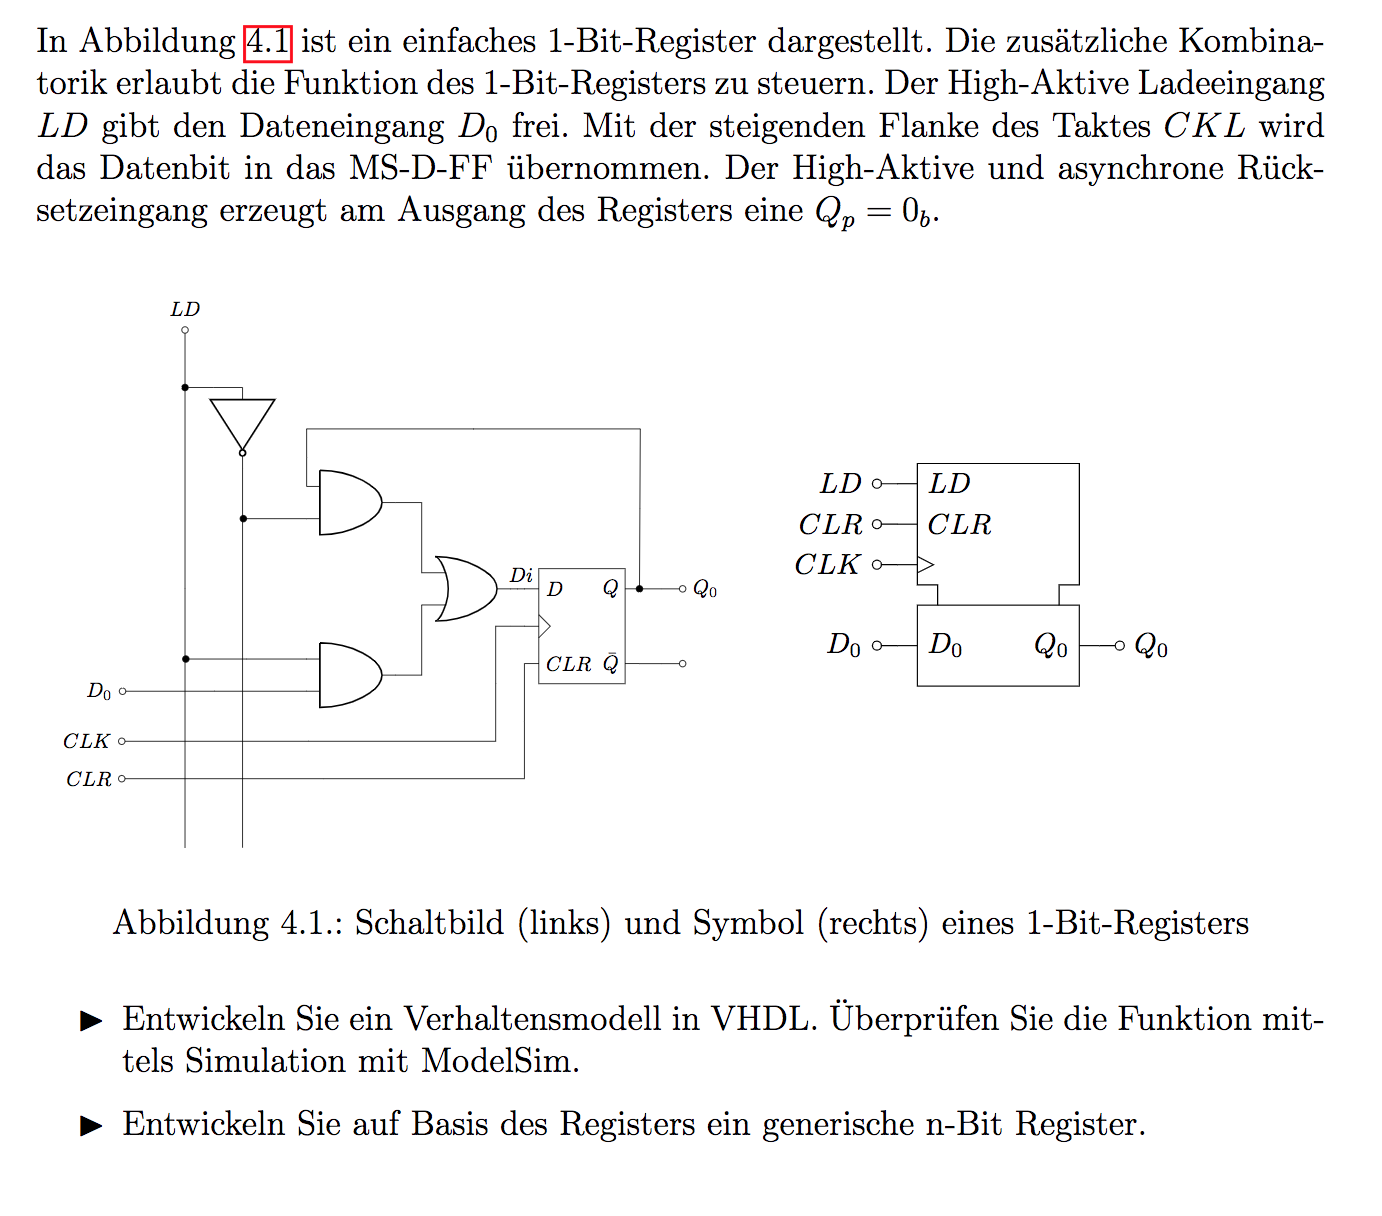
\includegraphics[width=0.8\textwidth]{411.png}}
\end{figure}

\lstinputlisting[language=vhdl, caption=One bit register VHDL Code]{./../Electronic_Design_Automation/Lab01_BasicComponents/one_bit_reg.vhd}

\lstinputlisting[caption=One-Bit Register Testbench]{./../Electronic_Design_Automation/Lab01_BasicComponents/tb_one_bit_reg.vhd}

\begin{figure}[!h]
	\centering
	\fbox{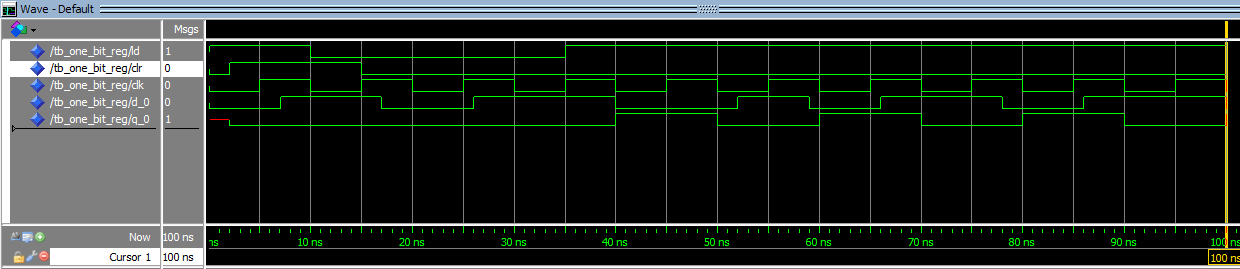
\includegraphics[width=1\textwidth]{./../Electronic_Design_Automation/Lab01_BasicComponents/one_bit_reg_simulation.png}}
		\captionof{figure}{On-Bit Register Modelsim Simulation}
\end{figure}

\lstinputlisting[caption=Generisches n-Bit Register]{./../Electronic_Design_Automation/Lab01_BasicComponents/n_bit_reg.vhd}

\lstinputlisting[caption=Generisches n-Bit Register Testbench]{./../Electronic_Design_Automation/Lab01_BasicComponents/tb_n_bit_reg.vhd}

\begin{figure}[!h]
	\centering
	\fbox{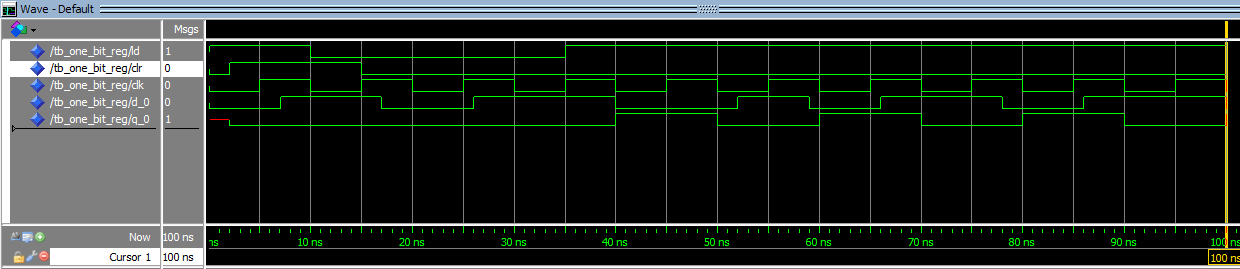
\includegraphics[width=1\textwidth]{./../Electronic_Design_Automation/Lab01_BasicComponents/one_bit_reg_simulation.png}}
	\captionof{figure}{One bit Register Modelsim Simulation}
\end{figure}

\newpage
\subsection{PIPO, SISO, PISO, SIPO}
Entwickeln Sie als Basiskomponenten folgende Register:
\begin{itemize}
\item Parallel-in / Parallel-out, PIPO
\item Parallel-in / Serial-out, PISO
\item Serial-in / Parallel-out, SIPO
\item Serial-in / Serial-out, SISO
\end{itemize}

=================================

\textbf{Parallel-in / Parallel-out, PIPO}
\lstinputlisting[caption=PIPO Register VHDL Code]{./../Electronic_Design_Automation/Lab01_BasicComponents/shift_pipo.vhd}

\lstinputlisting[caption=PIPO Register Testbench]{./../Electronic_Design_Automation/Lab01_BasicComponents/tb_shift_pipo.vhd}

\begin{figure}[!hb]
	\centering
	\fbox{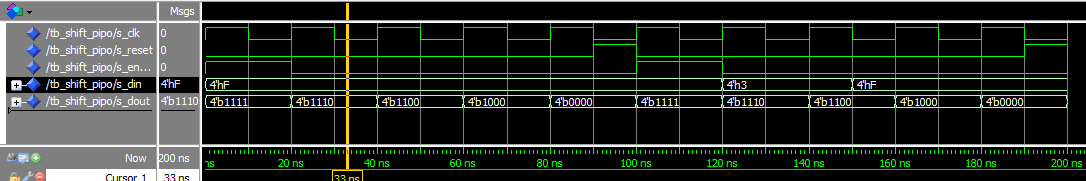
\includegraphics[width=1\textwidth]{./../Electronic_Design_Automation/Lab01_BasicComponents/shift_pipo_simulation.png}}
		\captionof{figure}{PIPO Register Modelsim Simulation}
\end{figure}

=================================

\textbf{Parallel-in / Serial-out, PISO}
\lstinputlisting[caption=PISO Register VHDL Code]{./../Electronic_Design_Automation/Lab01_BasicComponents/shift_piso.vhd}

\lstinputlisting[caption=PISO Register Testbench]{./../Electronic_Design_Automation/Lab01_BasicComponents/tb_shift_piso.vhd}

\begin{figure}[!hb]
	\centering
	\fbox{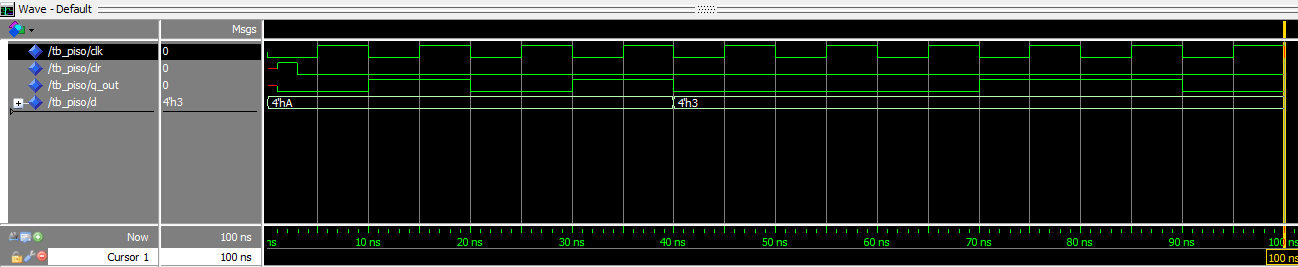
\includegraphics[width=1\textwidth]{./../Electronic_Design_Automation/Lab01_BasicComponents/shift_piso_simulation.png}}
		\captionof{figure}{PISO Register Modelsim Simulation}
\end{figure}


=================================

\textbf{Serial-in / Parallel-out, SIPO}
\lstinputlisting[caption=SIPO Register VHDL Code]{./../Electronic_Design_Automation/Lab01_BasicComponents/shift_sipo.vhd}

\lstinputlisting[caption=SIPO Register Testbench]{./../Electronic_Design_Automation/Lab01_BasicComponents/tb_shift_sipo.vhd}

\begin{figure}[!h]
	\centering
	\fbox{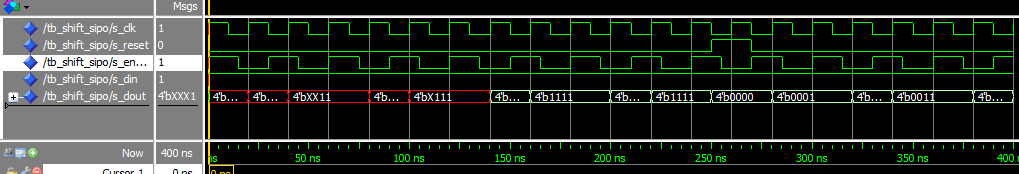
\includegraphics[width=1\textwidth]{./../Electronic_Design_Automation/Lab01_BasicComponents/shift_sipo_simulation.png}}
	\captionof{figure}{SIPO Register Modelsim Simulation}
\end{figure}

=================================

\textbf{Serial-in / Serial-out, SISO}
\lstinputlisting[caption=SISO Register VHDL Code]{./../Electronic_Design_Automation/Lab01_BasicComponents/shift_siso.vhd} 	

\lstinputlisting[caption=SISO Register Testbench]{./../Electronic_Design_Automation/Lab01_BasicComponents/tb_shift_siso.vhd}

\begin{figure}[!h]
	\centering
	\fbox{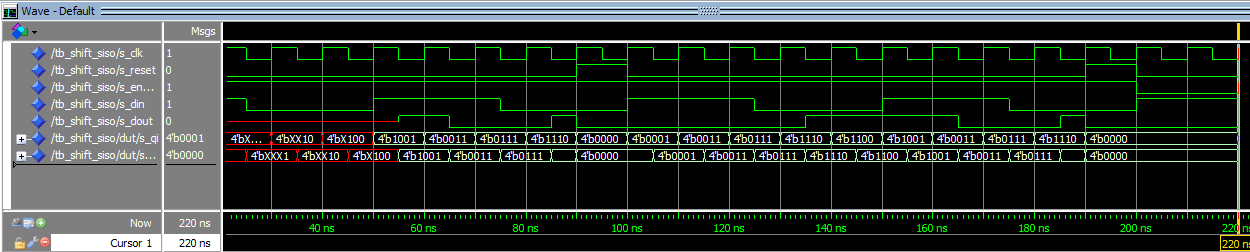
\includegraphics[width=1\textwidth]{./../Electronic_Design_Automation/Lab01_BasicComponents/shift_siso_simulation.png}}
		\captionof{figure}{SISO Register Modelsim Simulation}
\end{figure}


\subsection{4-Bit Universalregister}
\begin{figure}[!h]
	\centering
	\fbox{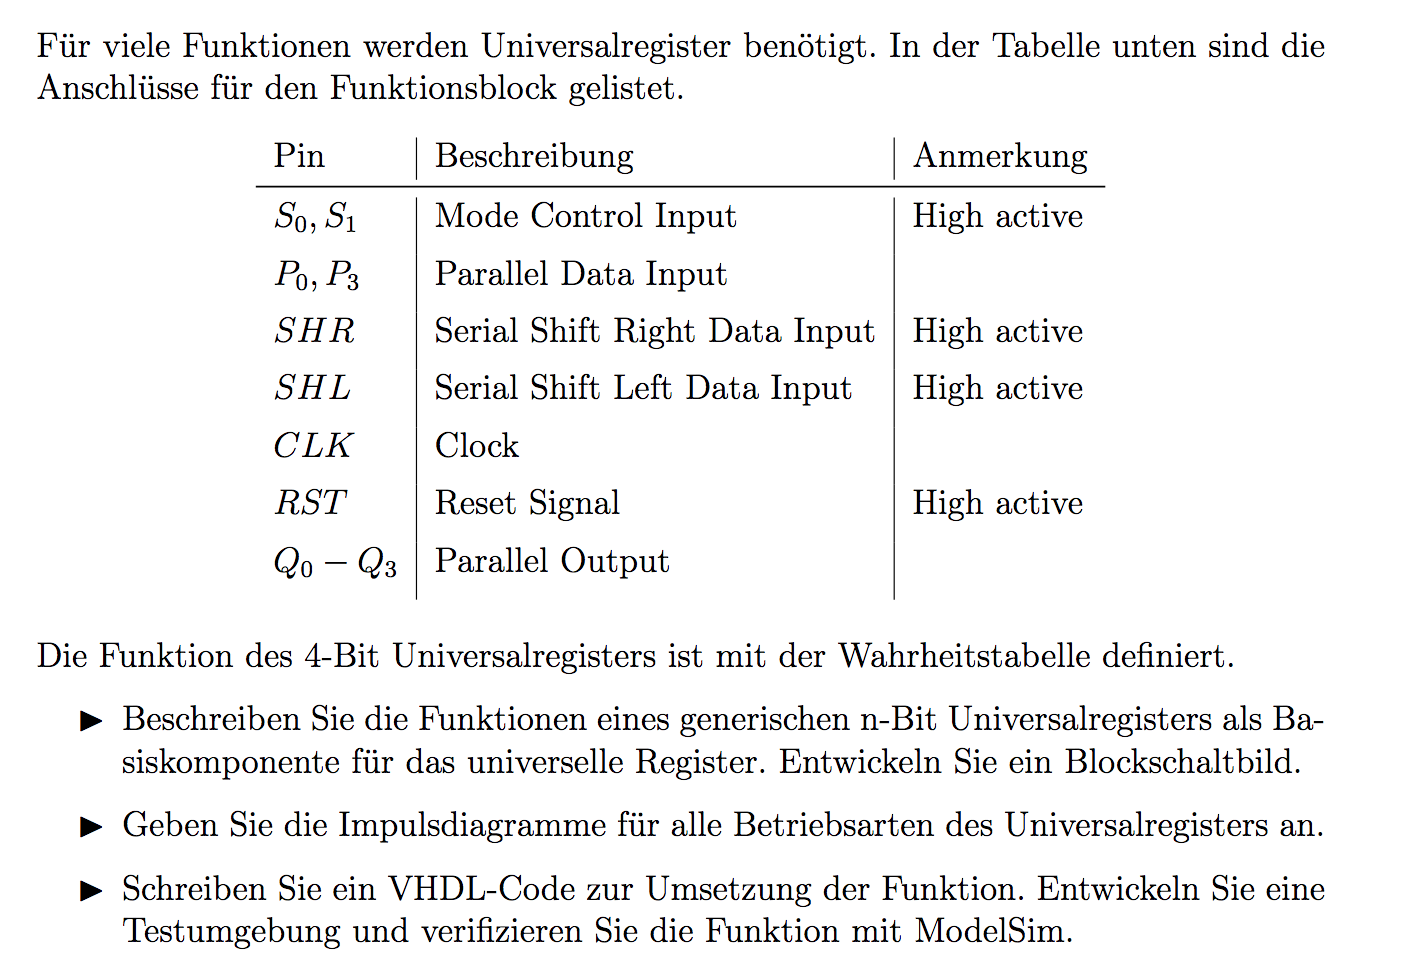
\includegraphics[width=0.8\textwidth]{413.png}}
\end{figure}

\lstinputlisting[caption=4-Bit  Universalregister VHDL Code]{./../Electronic_Design_Automation/Lab01_BasicComponents/shift_universal.vhd}

\lstinputlisting[caption=4-Bit  Universalregister Testbench]{./../Electronic_Design_Automation/Lab01_BasicComponents/tb_shift_universal.vhd}

\begin{figure}[!hb]
	\centering
	\fbox{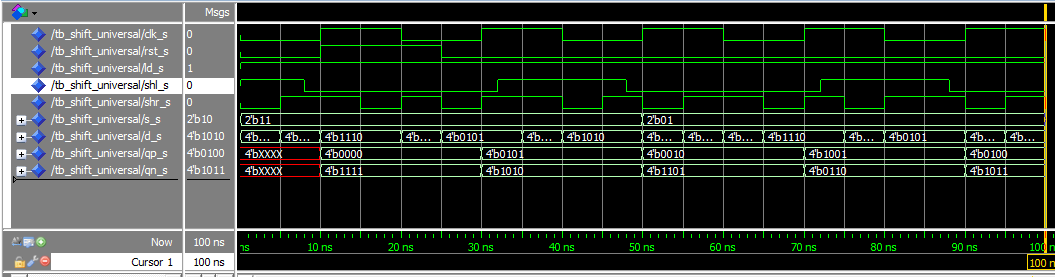
\includegraphics[width=1\textwidth]{./../Electronic_Design_Automation/Lab01_BasicComponents/shift_universal_simulation.png}}
		\captionof{figure}{4-Bit Register Modelsim Simulation}
\end{figure}

\newpage
\subsection{Arithmetik}
\begin{figure}[!hb]
	\centering
	\fbox{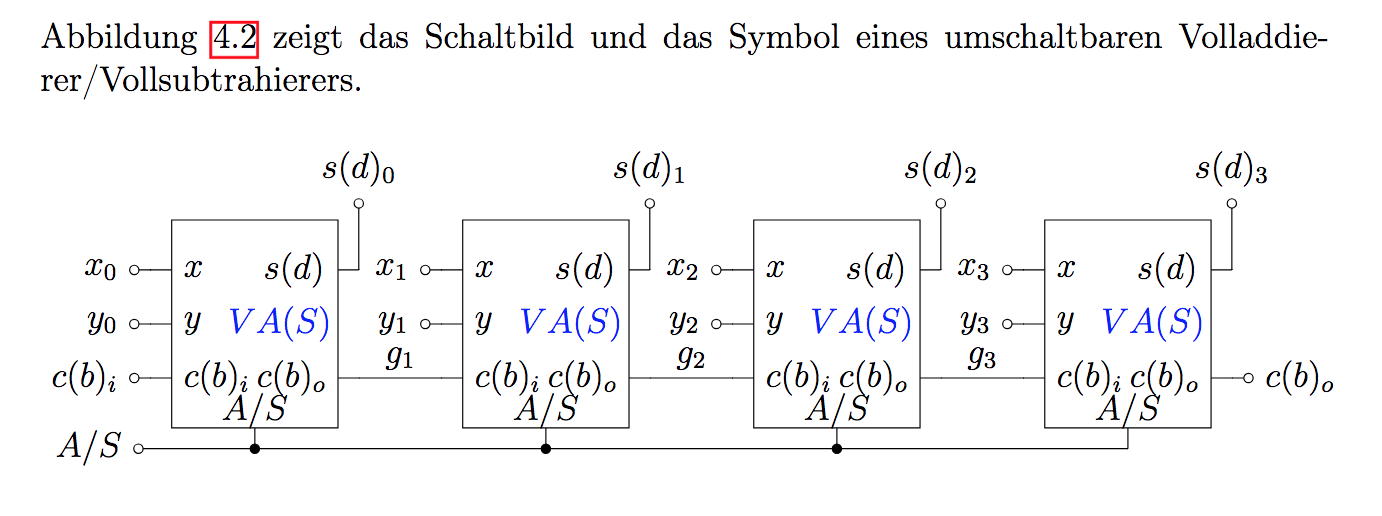
\includegraphics[width=0.8\textwidth]{414.png}}
\end{figure}

\lstinputlisting[caption=Full Adder VHDL code]{./../Electronic_Design_Automation/Lab01_BasicComponents/full_carry_ribble_adder.vhd}

\lstinputlisting[caption=Full Adder Testbench]{./../Electronic_Design_Automation/Lab01_BasicComponents/tb_full_carry_ribble_adder.vhd}

\begin{figure}[!ht]
	\centering
	\fbox{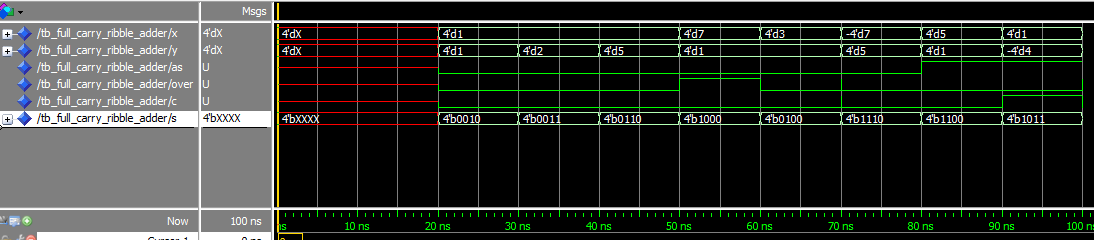
\includegraphics[width=1\textwidth]{./../Electronic_Design_Automation/Lab01_BasicComponents/full_adder_simulation.png}}
		\captionof{figure}{Full adder Modelsim Simulation}
\end{figure}

\newpage
\subsection{Siebensegmentanzeige}
Die Siebensegmentanzeige eignet sich auch zur Darstellung von Sedezimal-Code oder BCD-Codes. Zu entwerfen ist ein umschaltbarer Decoder gem�� der unten gegebenen Wahrheitstabelle
\begin{figure}[!h]
	\centering
	\fbox{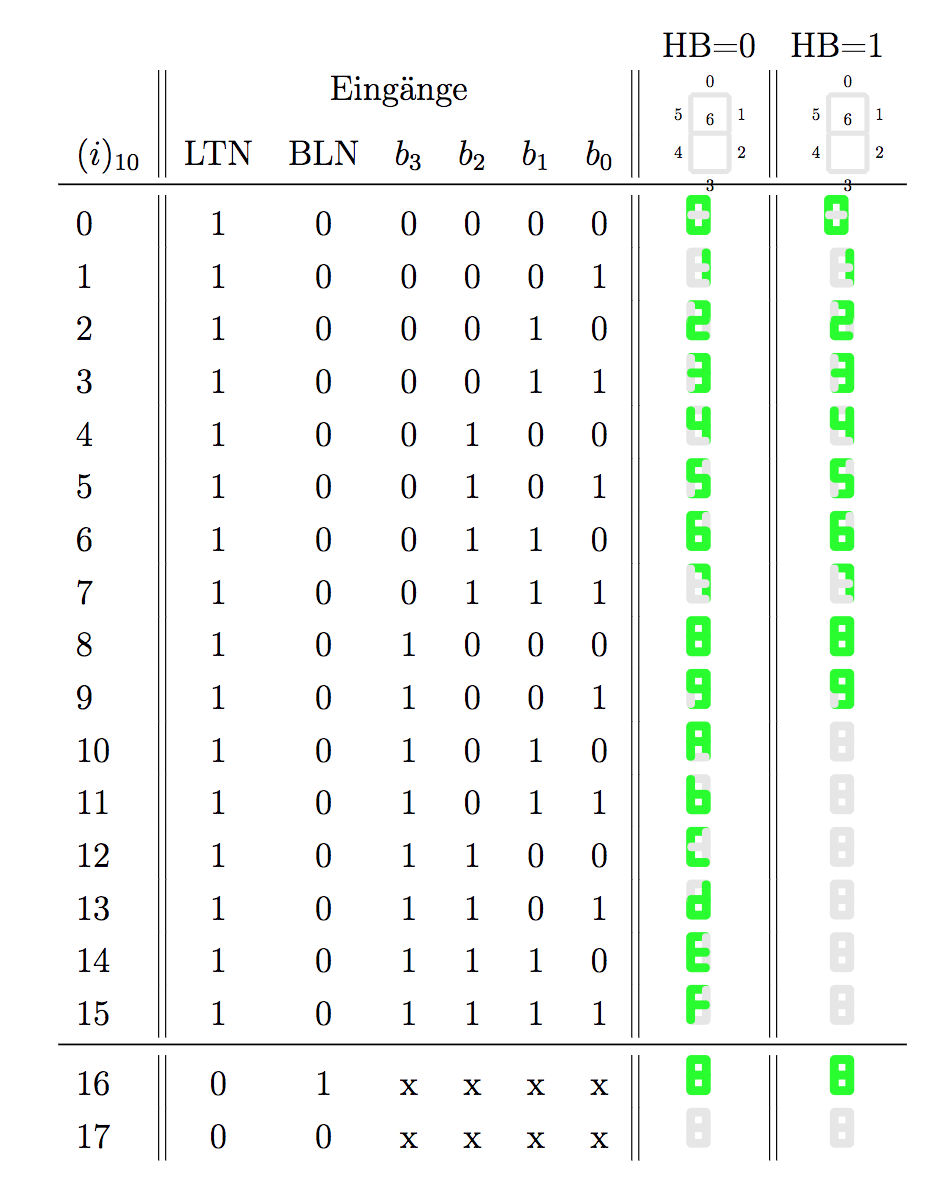
\includegraphics[width=0.6\textwidth]{415.png}}
\end{figure}

\lstinputlisting[caption=Seven segment display VHDL code]{./../Electronic_Design_Automation/Lab01_BasicComponents/seven_seg.vhd}

\lstinputlisting[caption=Seven segment display Testbench]{./../Electronic_Design_Automation/Lab01_BasicComponents/tb_seven_seg.vhd}

\begin{figure}[!ht]
	\centering
	\fbox{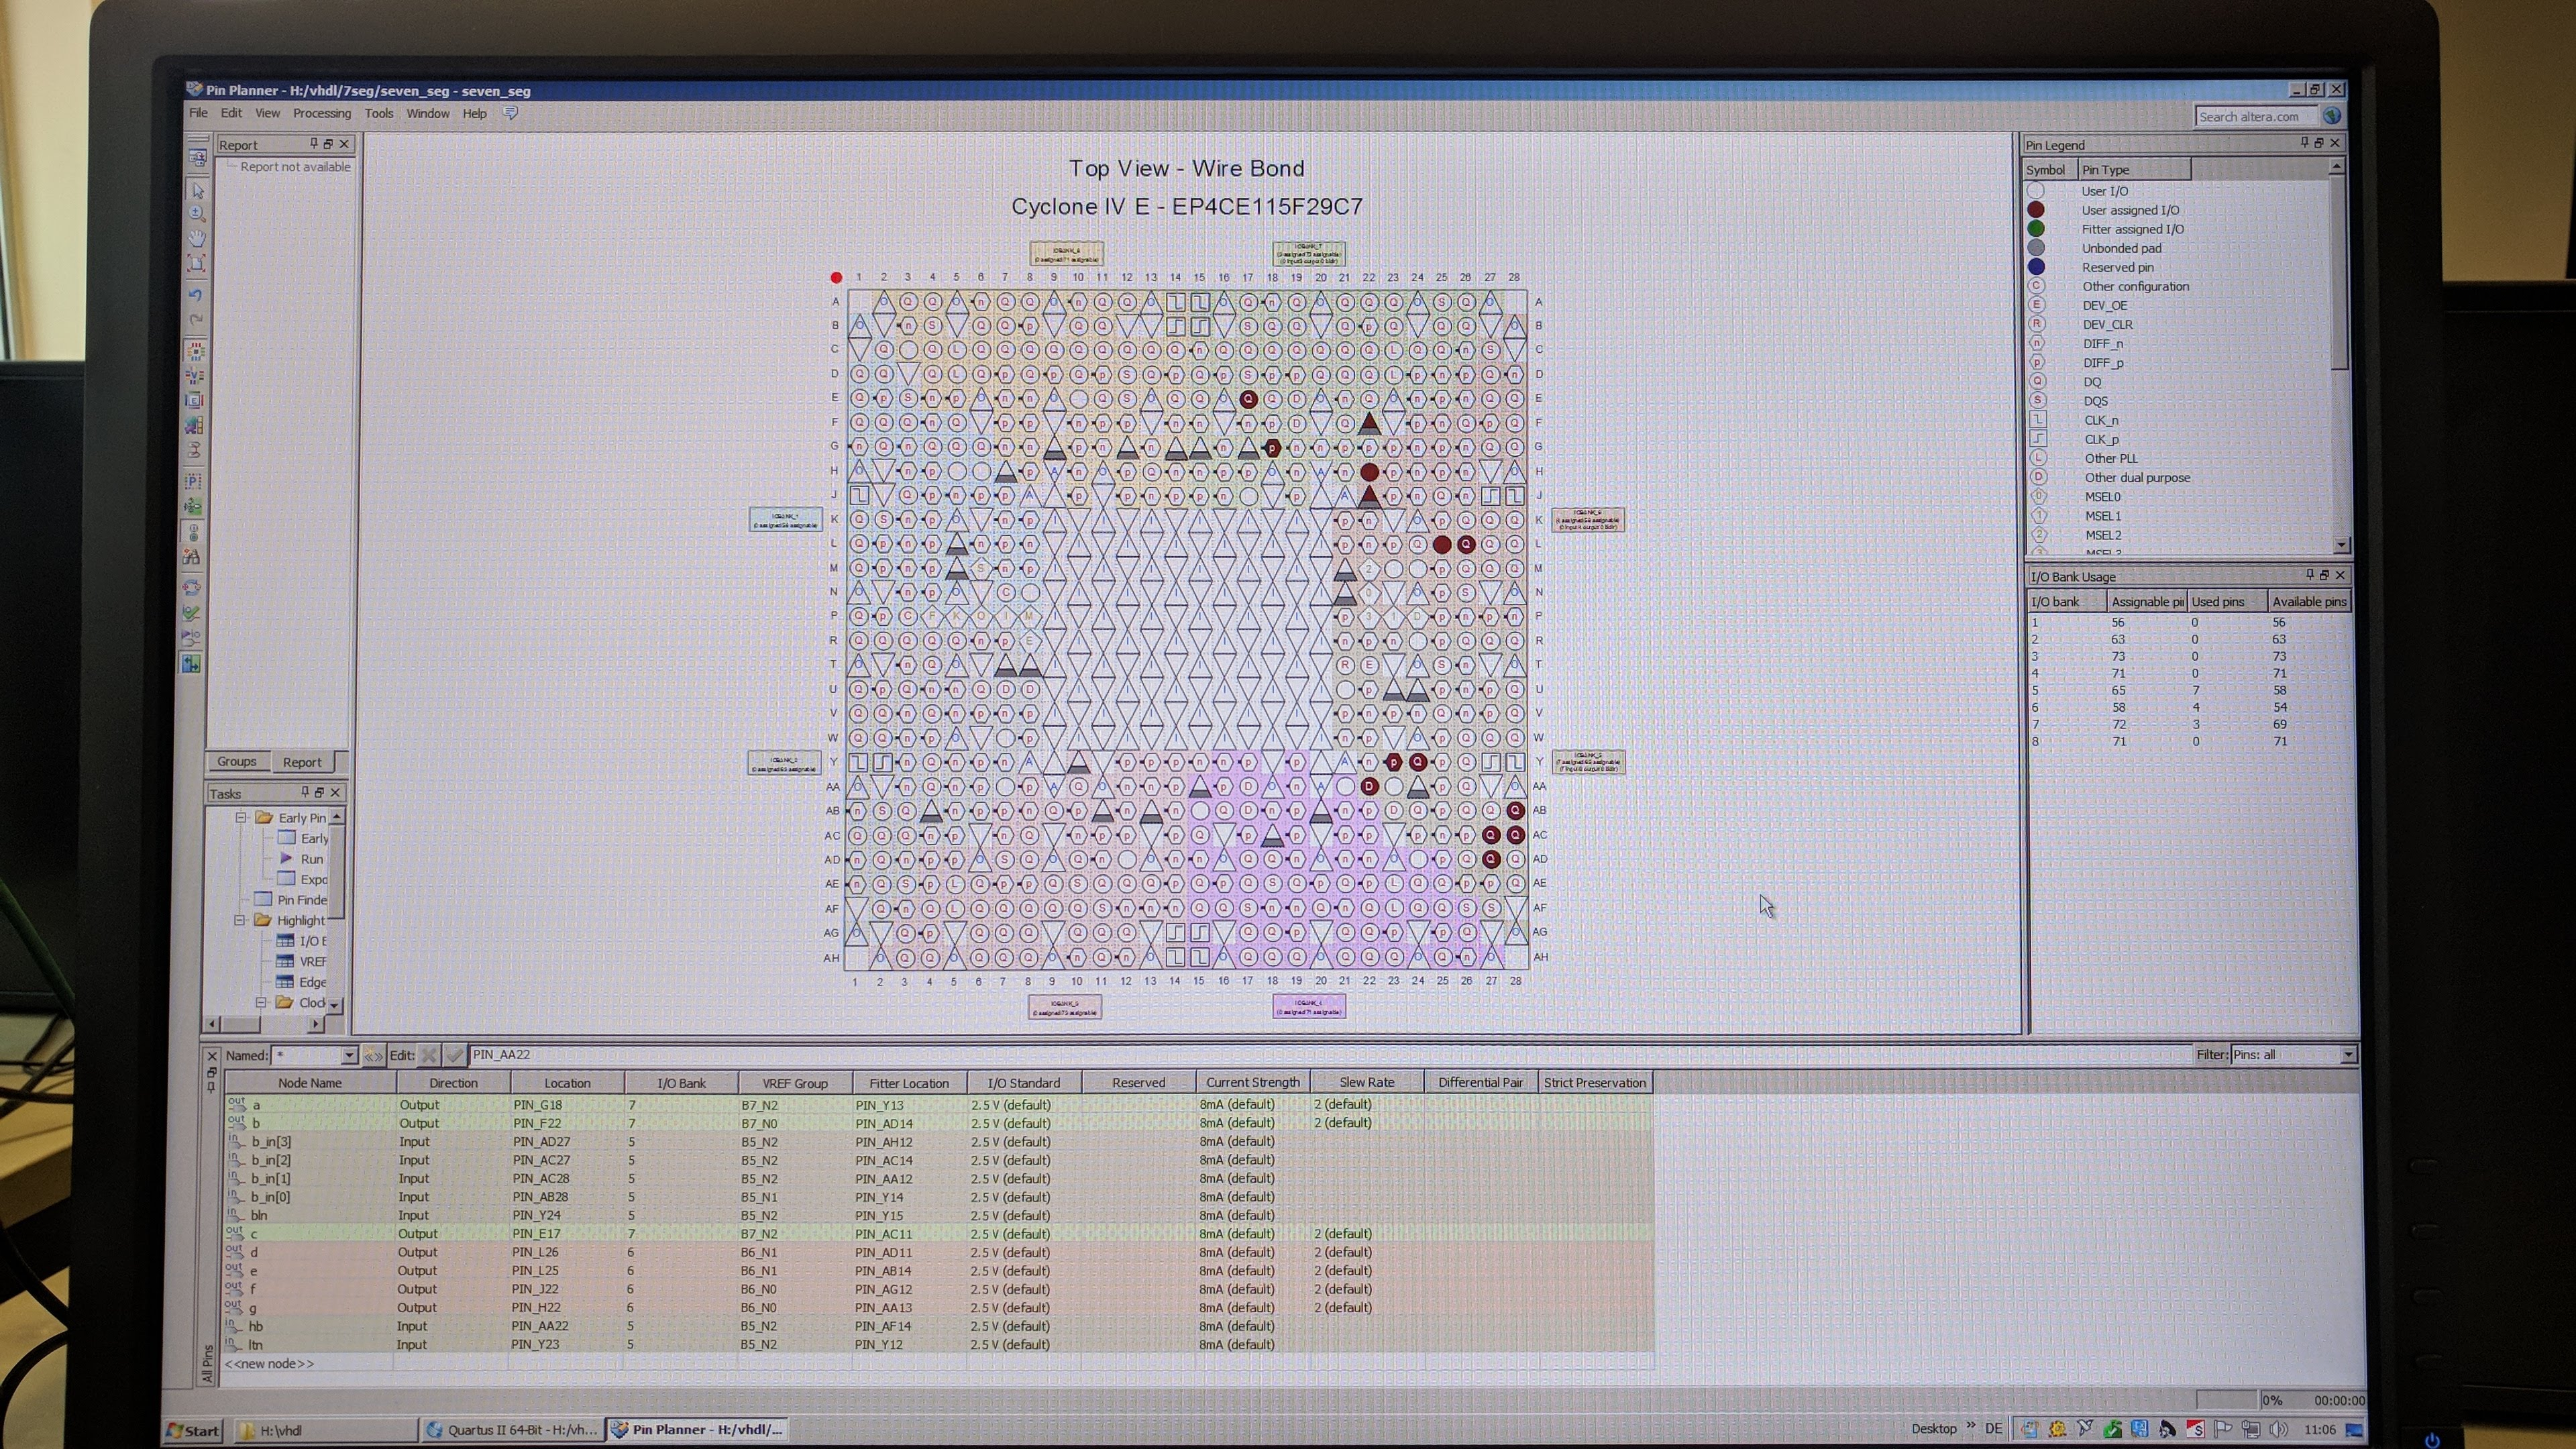
\includegraphics[width=0.6\textwidth]{seven01.jpg}}
	\captionof{figure}{Ausf�hrung auf dem Entwicklungsboard DE2-115}
\end{figure}
\begin{figure}[!h]
	\centering
	\fbox{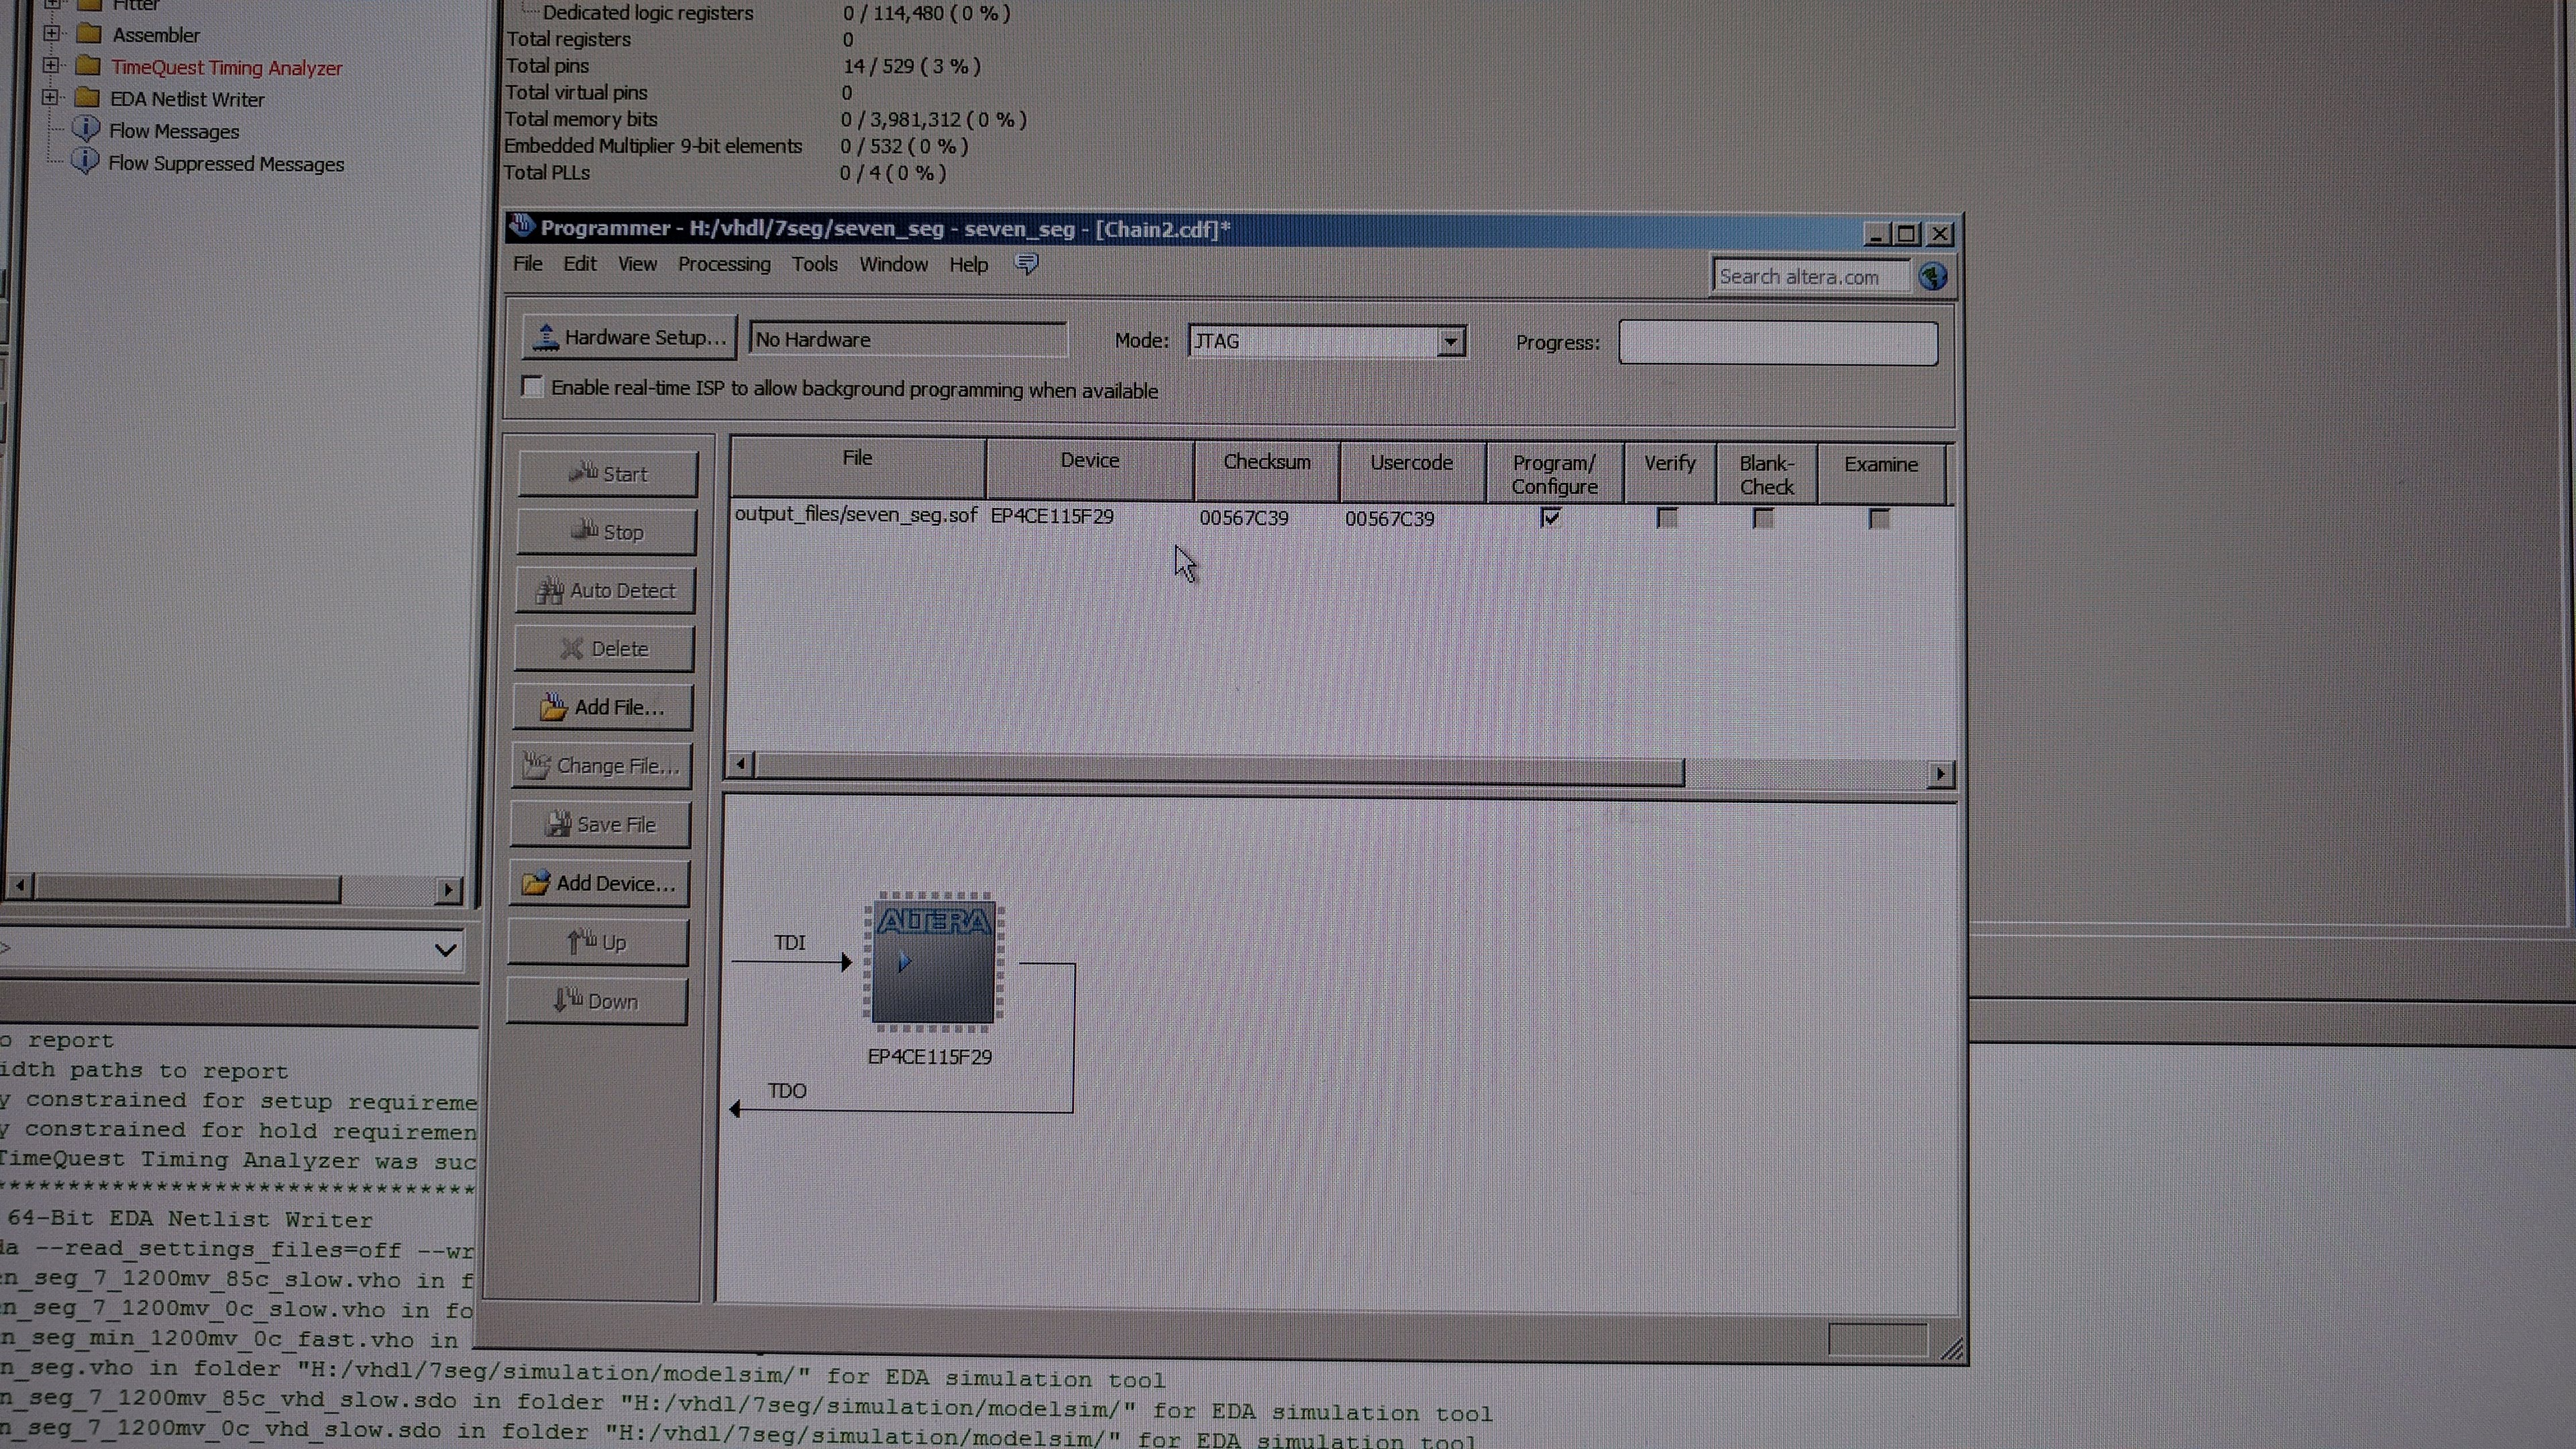
\includegraphics[width=0.6\textwidth]{seven02.jpg}}
	\captionof{figure}{Ausf�hrung auf dem Entwicklungsboard DE2-115n}
\end{figure}
\begin{figure}[!h]
	\centering
	\fbox{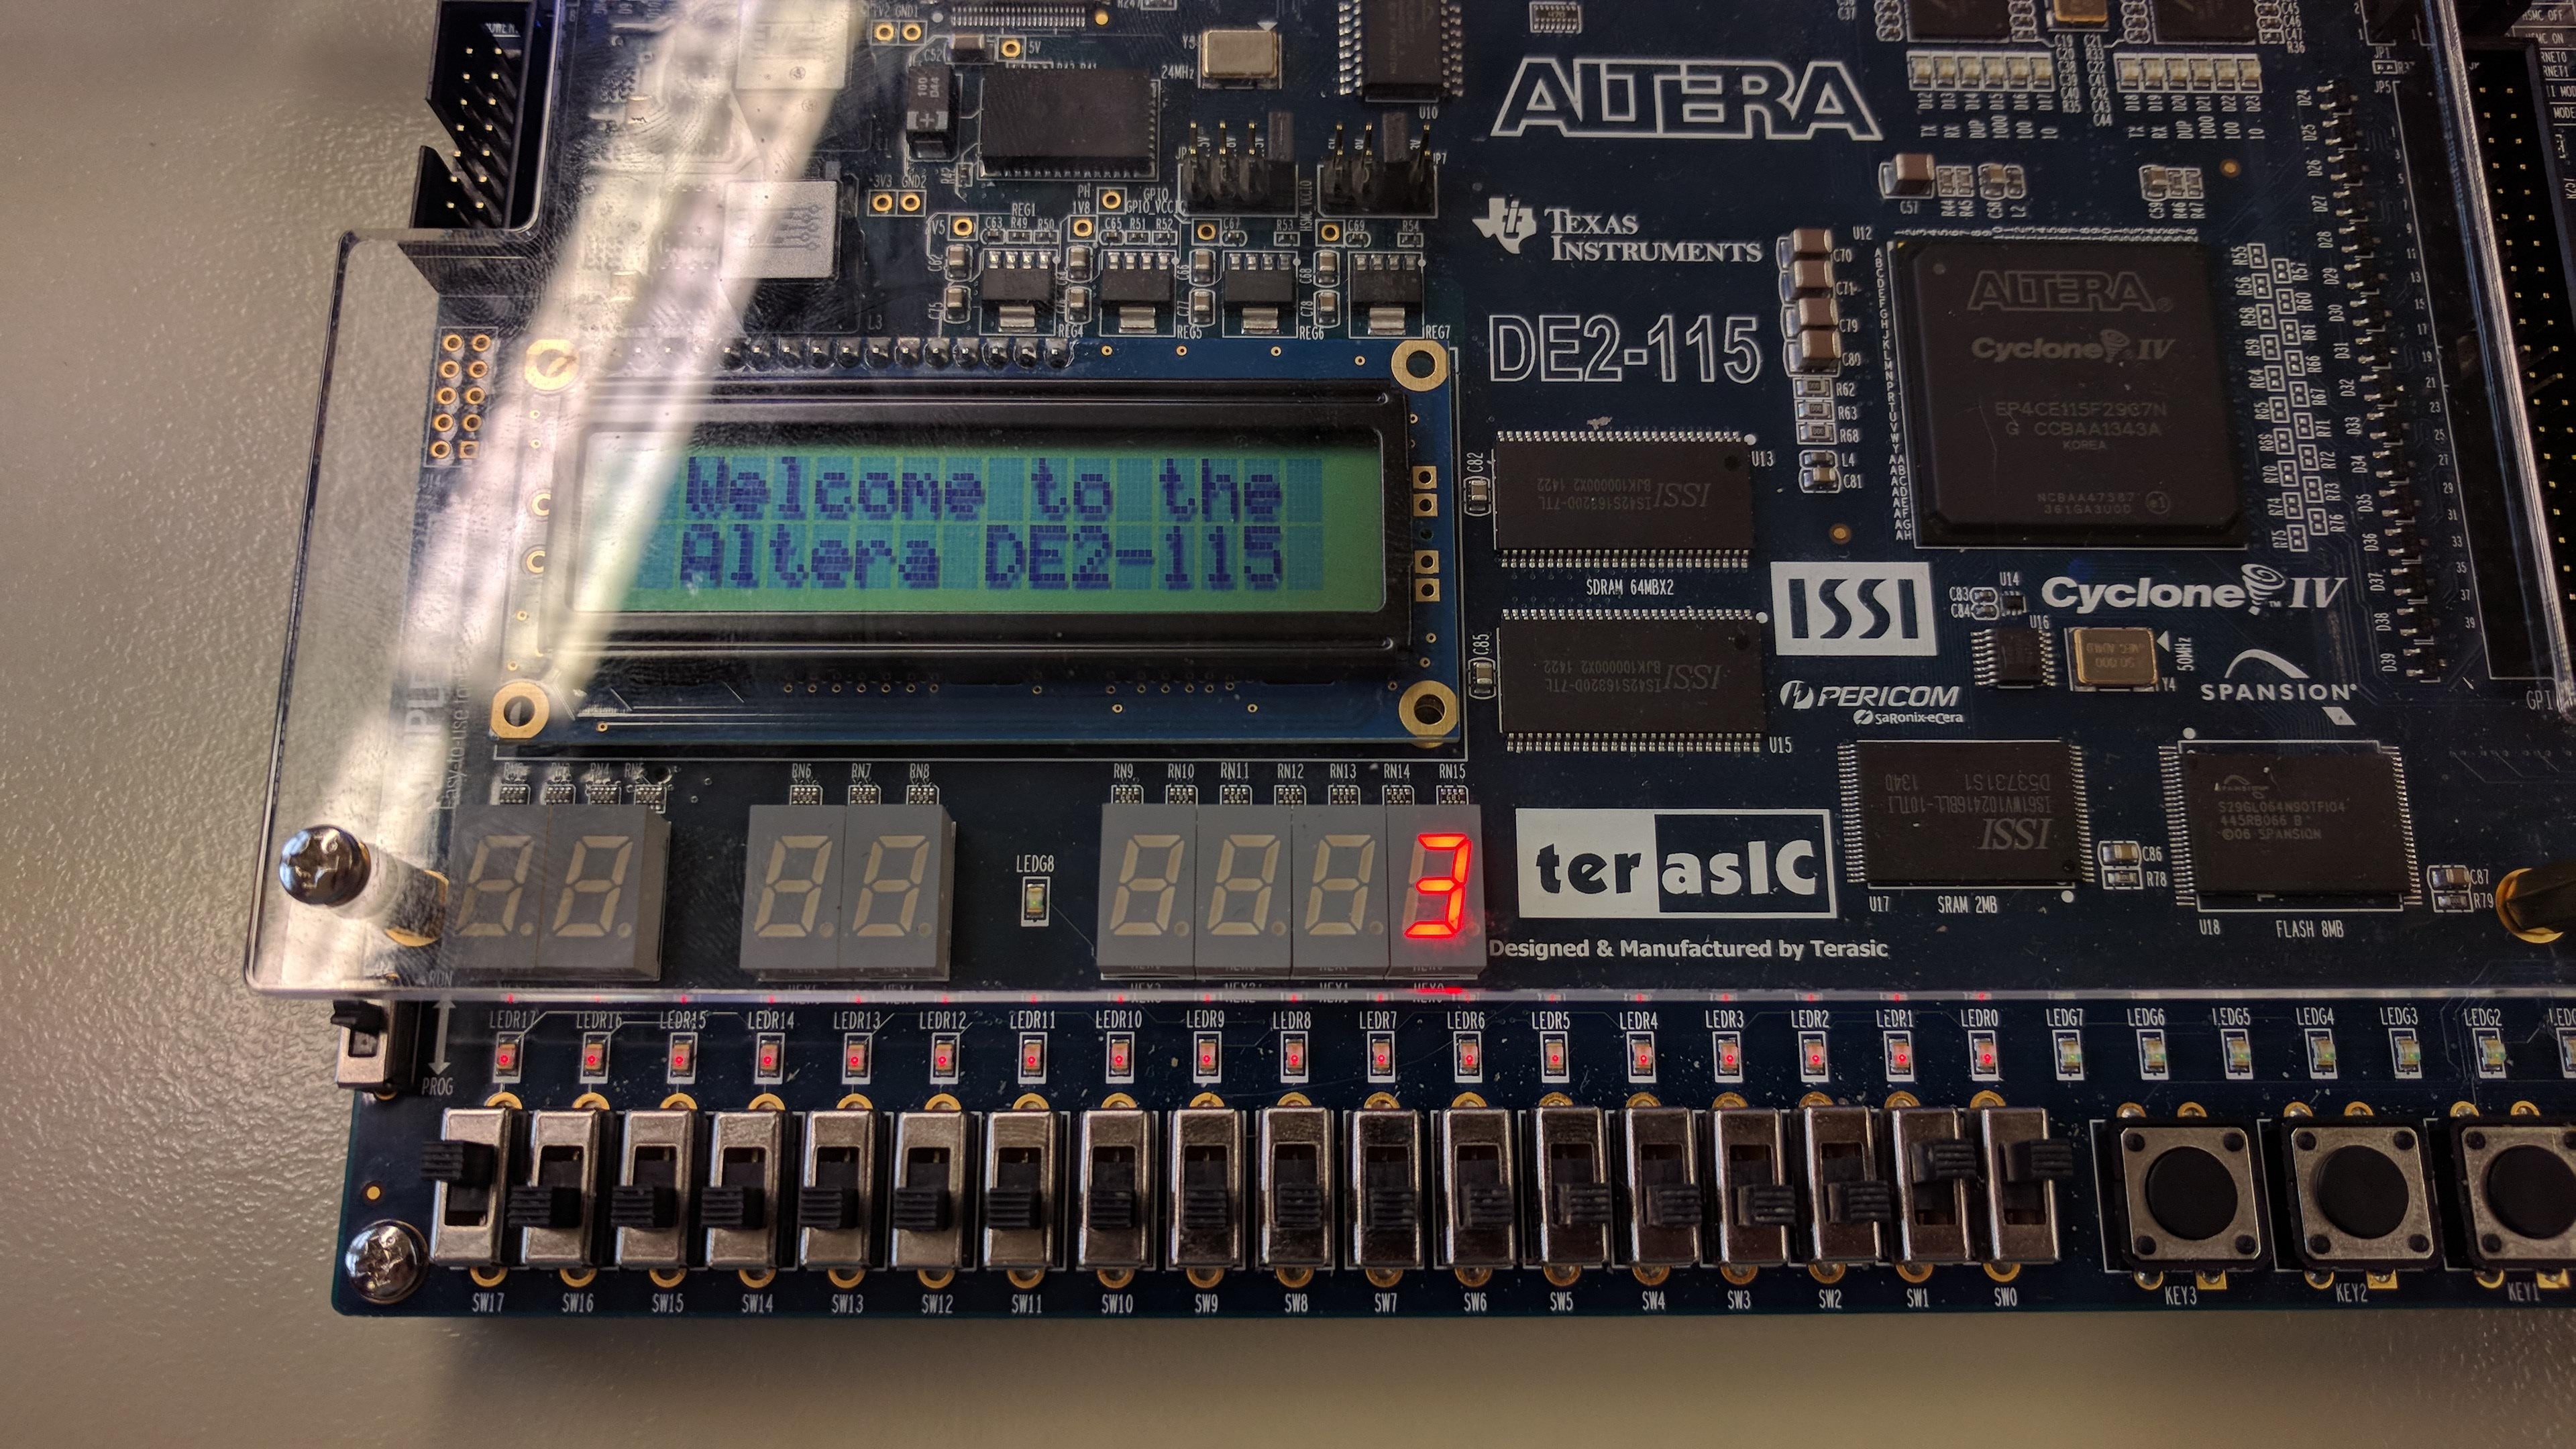
\includegraphics[width=0.6\textwidth]{seven03.jpg}}
	\captionof{figure}{Ausf�hrung auf dem Entwicklungsboard DE2-115}
\end{figure}
\begin{figure}[!h]
	\centering
	\fbox{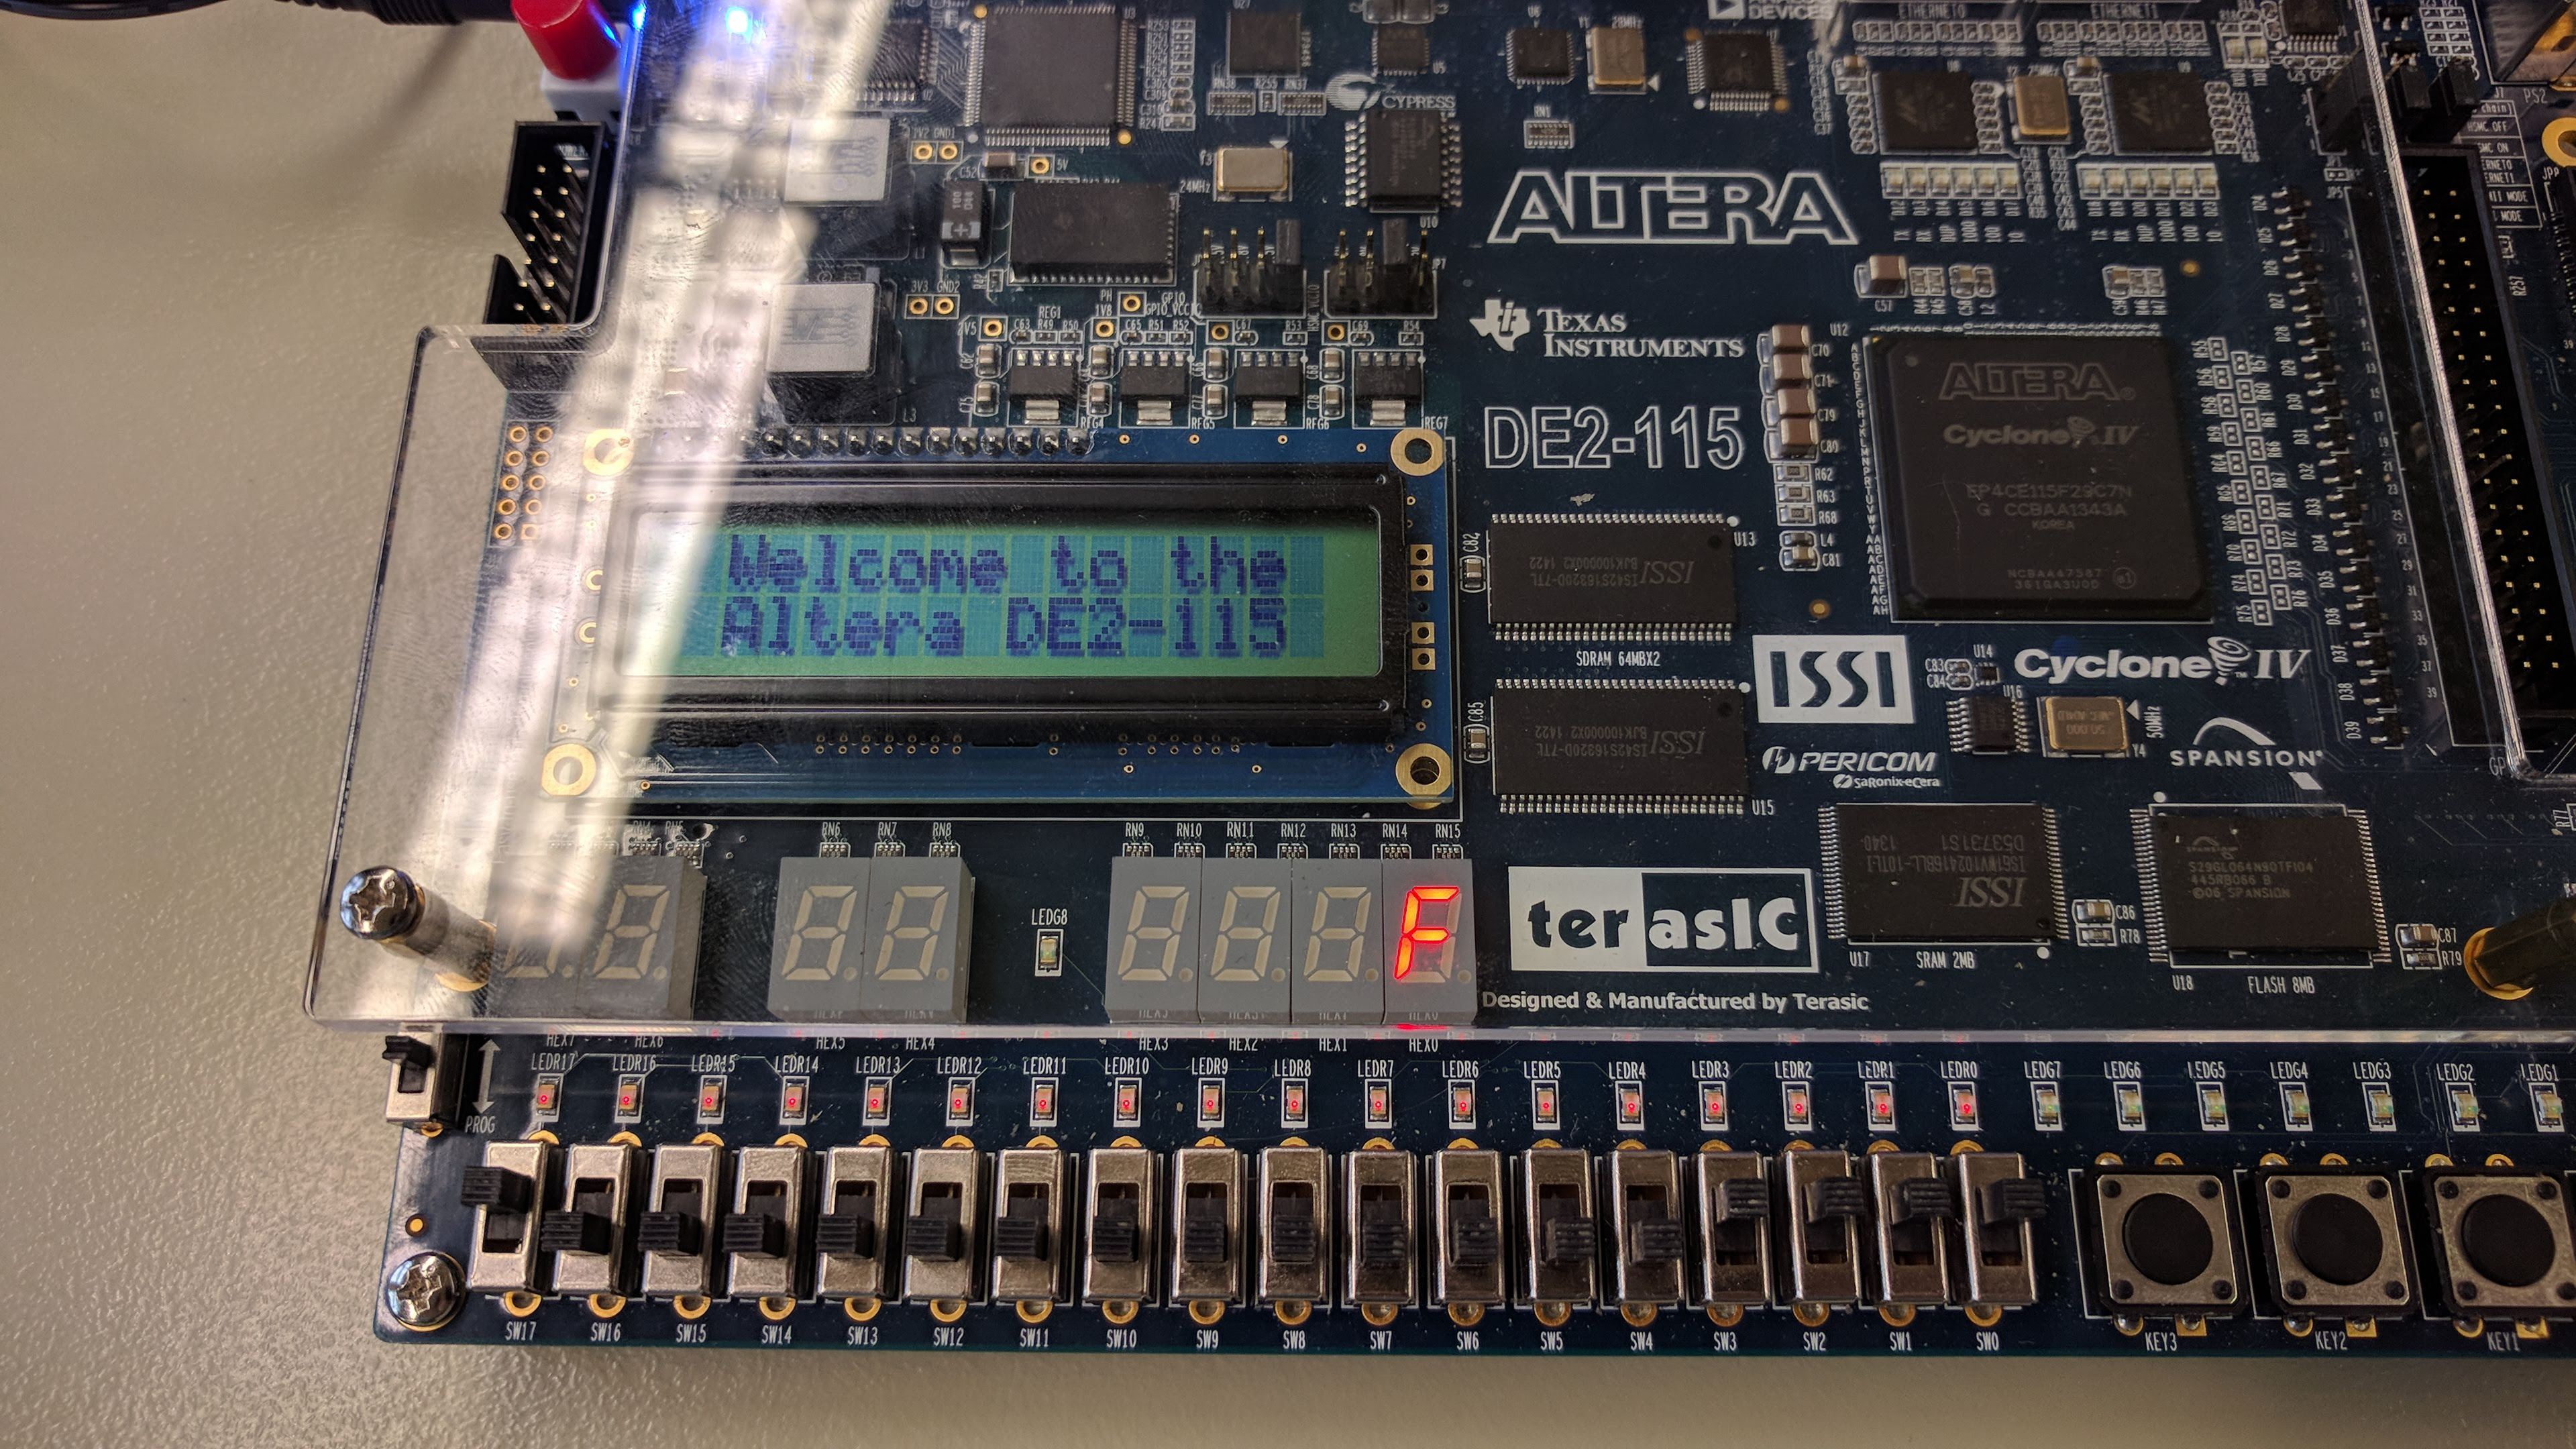
\includegraphics[width=0.6\textwidth]{seven04.jpg}}
	\captionof{figure}{Ausf�hrung auf dem Entwicklungsboard DE2-115}
\end{figure}
\begin{figure}[!h]
	\centering
	\fbox{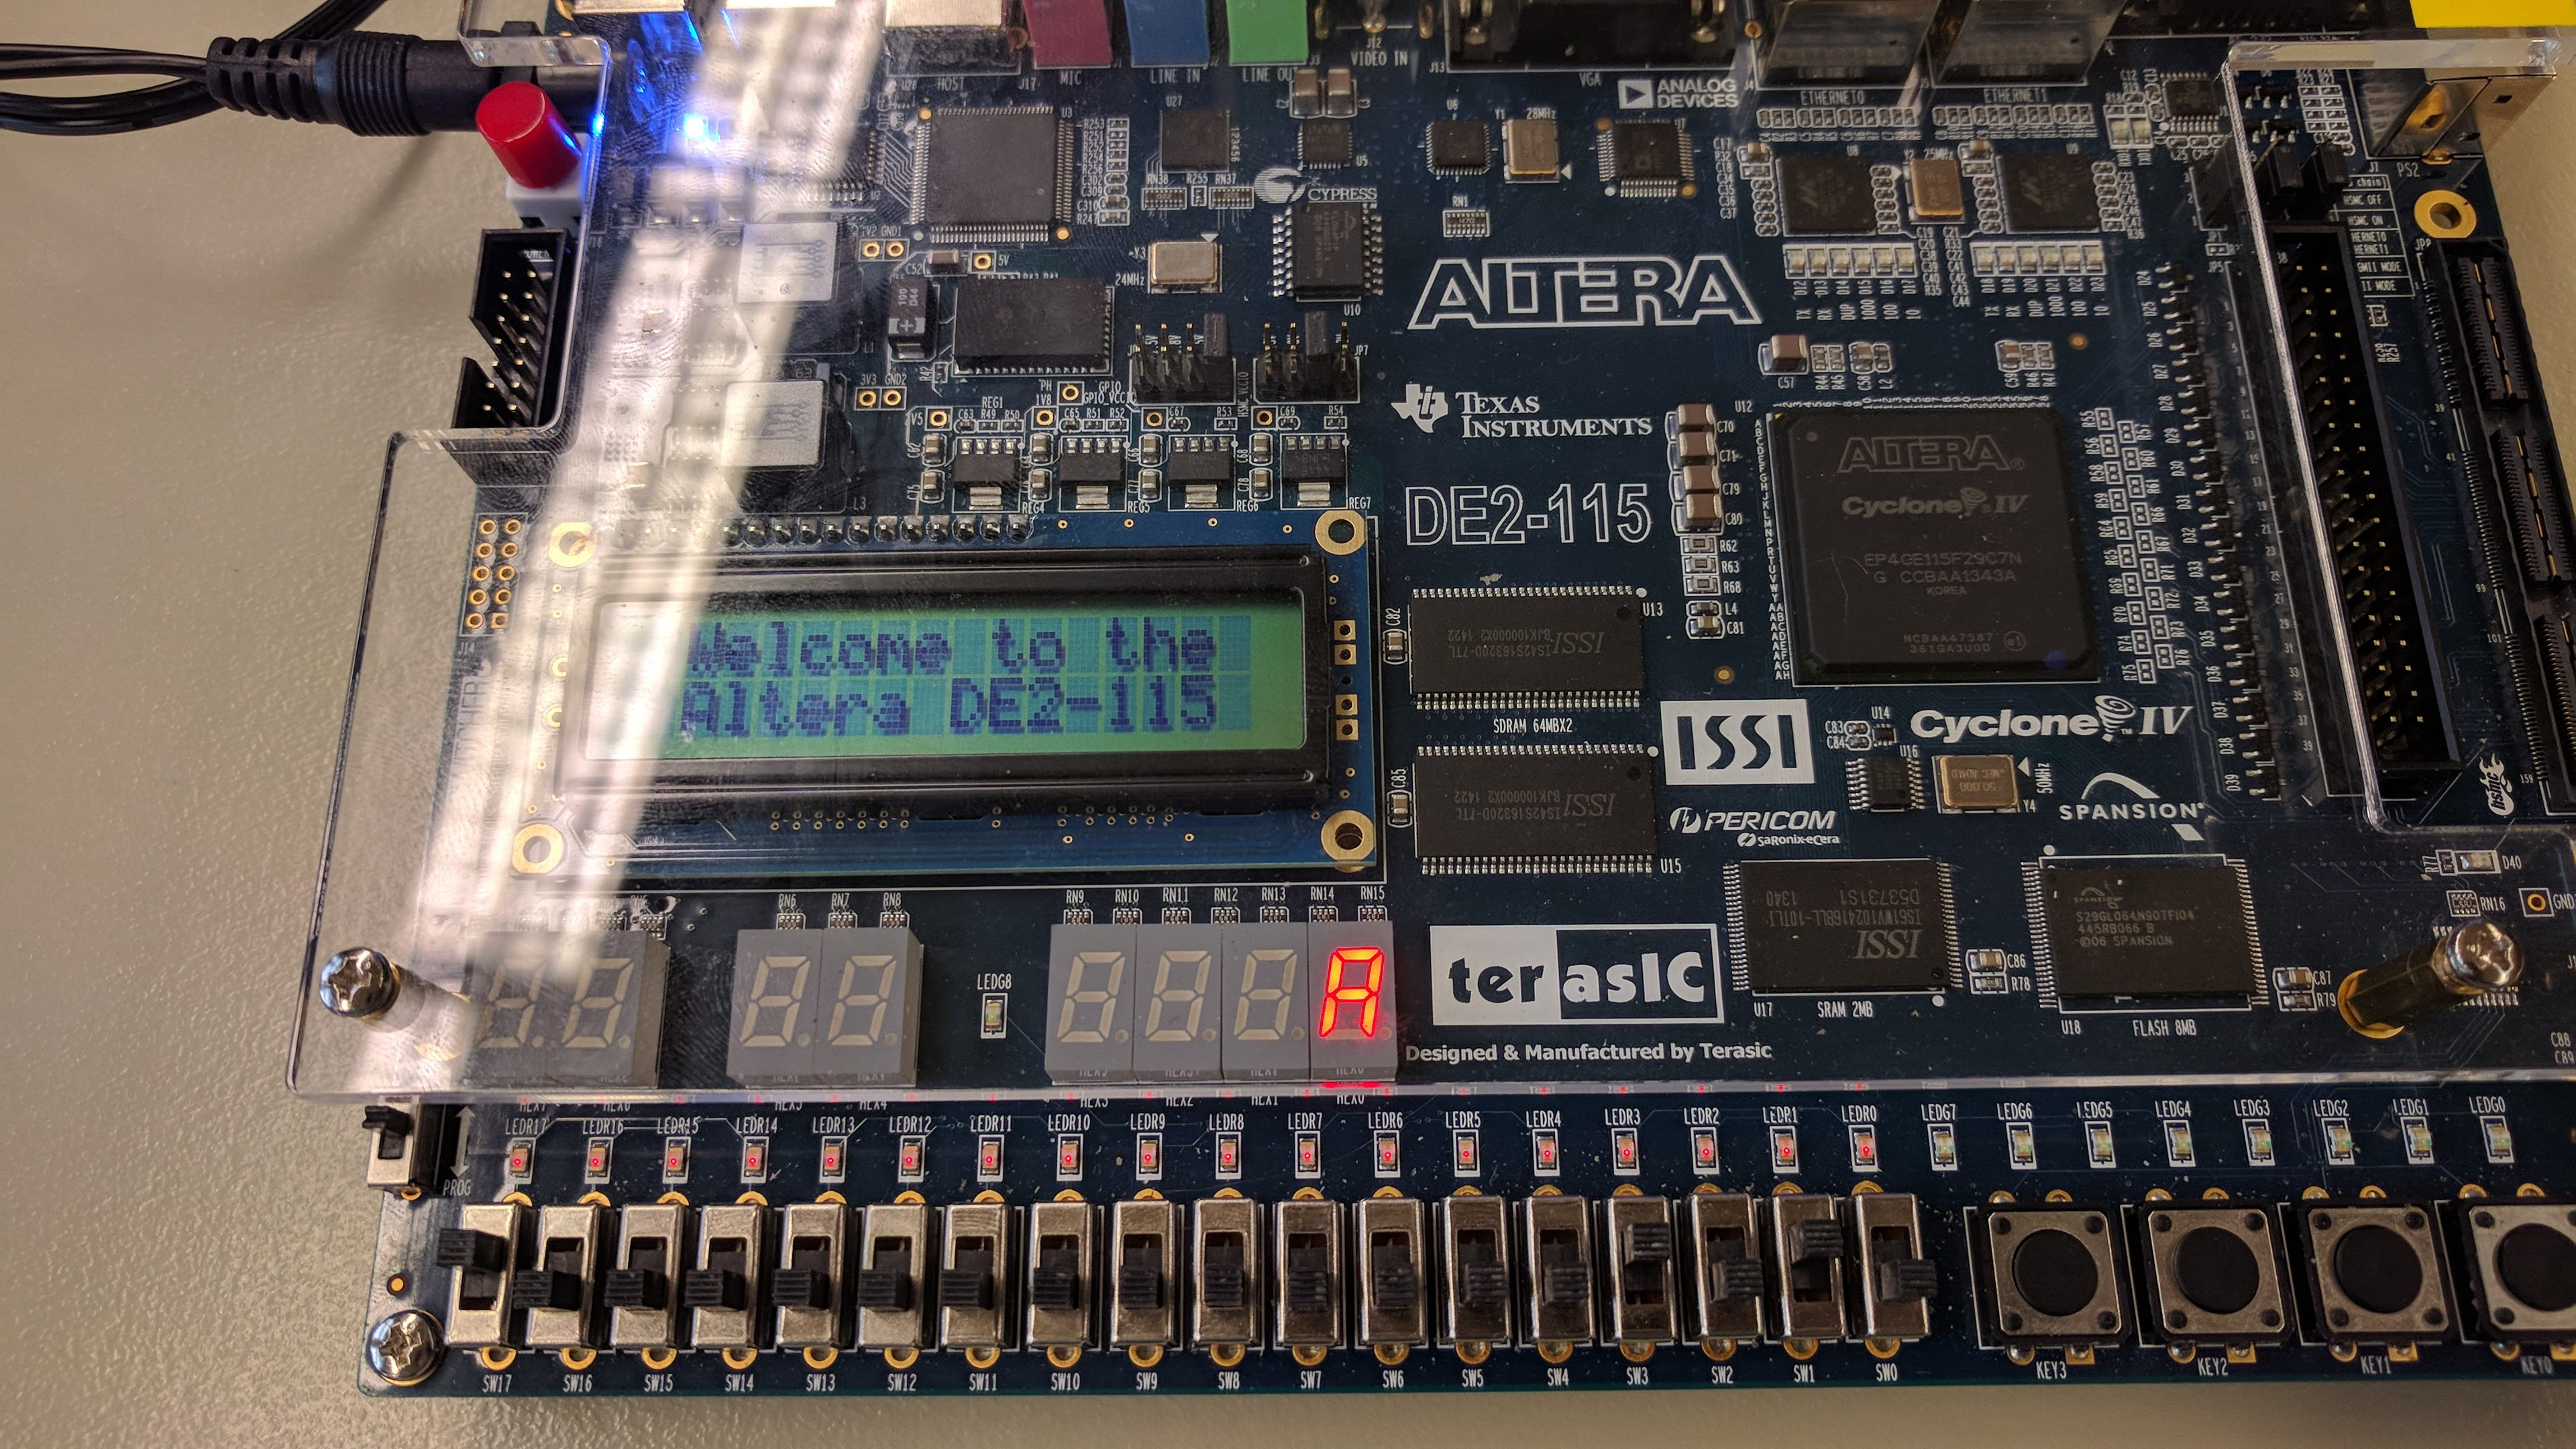
\includegraphics[width=0.6\textwidth]{seven05.jpg}}
	\captionof{figure}{Ausf�hrung auf dem Entwicklungsboard DE2-115}
\end{figure}

\clearpage
\section{Laboraufgaben: 2. Erkennung einer Bit-Sequenz}
\begin{figure}[h]
	\centering
	\begin{tikztimingtable}
		{CLK} & LHLHLHLHLHLHLHLHLHLHLHLHLHLHLHLH \\ %32
		{RESET} & XLHHHHHHHHHHHHHHHHHHHHHHHHHHHHHH \\
		{x} & XLLLLHHLLLLLLLLHHHHHHHHHHLLLLLLL \\
		{y} & XLLLLLLLLLLLLLLHHLLLLLLHHHHLLLLL \\
	\end{tikztimingtable}
	\caption{Impulsdiagramm des Zustandsautomaten zur Bit-Sequenzerkennung}\label{fig:impulse}
\end{figure}

\begin{figure}[h]
	\centering
	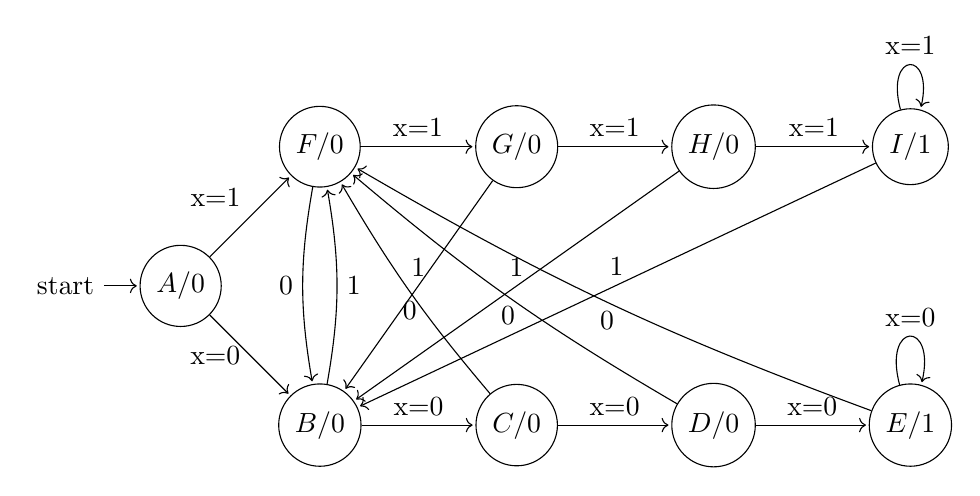
\begin{tikzpicture}[shorten >=1pt,node distance=2.5cm,on grid,auto] 
	\node[state,initial] (a)   {$A/0$};
	\node[state] (f) [above right=of a] {$F/0$};
	\node[state] (g) [right=of f] {$G/0$};
	\node[state] (h) [right=of g] {$H/0$};
	\node[state] (i) [right=of h] {$I/1$};    
	\node[state] (b) [below right=of a] {$B/0$};
	\node[state] (c) [right=of b] {$C/0$};
	\node[state] (d) [right=of c] {$D/0$};
	\node[state] (e) [right=of d] {$E/1$};   
	\path[->]
	(a) edge node {x=1} (f)
	(f) edge node {x=1} (g)
	(g) edge node {x=1} (h)
	(h) edge node {x=1} (i)
	(i) edge [loop above] node {x=1} (i)
	(a) edge node [left] {x=0} (b)
	(b) edge node {x=0} (c)
	(c) edge node {x=0} (d)
	(d) edge node {x=0} (e)
	(e) edge [loop above] node {x=0} (e)    
	(b) edge [bend right=10] node [right] {1} (f)
	(f) edge [bend right=10] node [left] {0} (b)
	(c) edge [bend left=5] node [below] {0} (f)    
	(d) edge [bend left=5] node [below] {0} (f)
	(e) edge [bend left=5] node [below] {0} (f)
	(g) edge node [above] {1} (b)
	(h) edge node [above] {1} (b)
	(i) edge node [above] {1} (b)	
	;
	\end{tikzpicture}
	\caption{Zustandsdiagramm zur Erkennung einer gleichf�rmigen Bit-Sequenz}\label{fig:state}
\end{figure}

\subsection{Aufgabenstellungen A}

\lstinputlisting[caption=State Machine VHDL Code]{./../Electronic_Design_Automation/Lab02_BitSequence/bit_seq_ff_v1.vhd}

\lstinputlisting[caption=State Machine Testbench]{./../Electronic_Design_Automation/Lab02_BitSequence/tb_bit_seq.vhd}

\begin{figure}[!hb]
	\centering
	\fbox{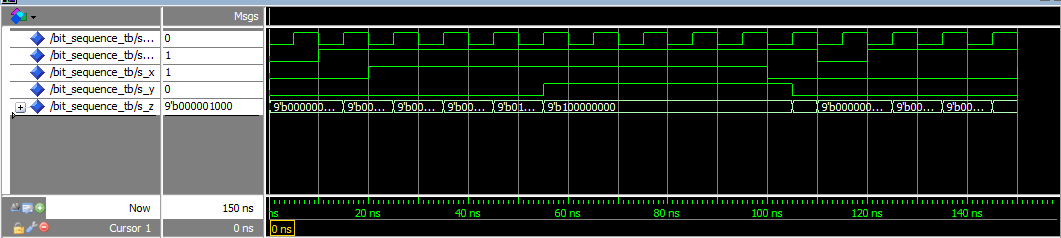
\includegraphics[width=1\textwidth]{./../Electronic_Design_Automation/Lab02_BitSequence/bit_sequence_simulation_a.png}}
	\captionof{figure}{State Machine Modelsim Simulation}
\end{figure}

\clearpage
\subsection{Aufgabenstellungen B}
\lstinputlisting[caption=State Machine VHDL Code]{./../Electronic_Design_Automation/Lab02_BitSequence/bit_seq_ff_v2.vhd}

\lstinputlisting[caption=State Machine Testbench]{./../Electronic_Design_Automation/Lab02_BitSequence/tb_bit_seq.vhd}

\begin{figure}[!hb]
	\centering
	\fbox{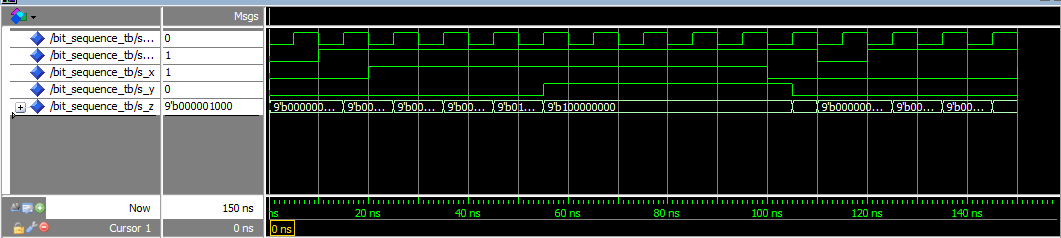
\includegraphics[width=1\textwidth]{./../Electronic_Design_Automation/Lab02_BitSequence/bit_sequence_simulation_a.png}}
	\captionof{figure}{State Machine Modelsim Simulation}
\end{figure}

\clearpage
\subsection{Aufgabenstellungen C}
\lstinputlisting[caption=State Machine VHDL Code]{./../Electronic_Design_Automation/Lab02_BitSequence/bit_sequence_b.vhd}

\lstinputlisting[caption=State Machine Testbench]{./../Electronic_Design_Automation/Lab02_BitSequence/bit_sequence_b_tb.vhd}

\begin{figure}[!hb]
	\centering
	\fbox{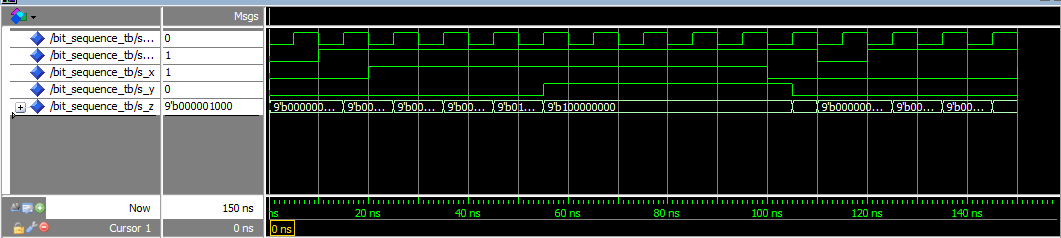
\includegraphics[width=1\textwidth]{./../Electronic_Design_Automation/Lab02_BitSequence/bit_sequence_simulation_a.png}}
	\captionof{figure}{State Machine Modelsim Simulation}
\end{figure}

\clearpage
\section{Laboraufgaben: 3. Takte, Z�hler und Zeitgeber}
\subsection{BCD-Z�hler und Codierung}
In Abbildung \ref{fig:l3-scd} ist das vereinfachte Systemschaltbild zur Aufgabenstellung dargestellt. Der BCD-Counter kann �ber die Schalter auf dem Entwicklungsbord initialisiert werden (Startwerteingabe). Der Z�hlerstand soll sowohl auf einer Siebensegmentanzeige dargestellt als auch auf dem LCD-Display (siehe Abbildung \ref{fig:l3-lcd}) angezeigt werden.

\begin{figure}[H]
	\centering
	
\includegraphics[width=.6\textwidth,
	page=61,
	trim=4cm 4.6cm 3.5cm 15.5cm,
	clip]
	{Labor_PL_Gregorius.pdf}
	\caption{L3 Systemschaltbild zur Aufgabenstellung}
	\label{fig:l3-scd}
\end{figure}

\begin{minipage}[b]{.49\textwidth}
	\begin{figure}[H]
		
\includegraphics[width=\textwidth,
		page=61,
		trim=4cm 18cm 4cm 5cm,
		clip]
		{Labor_PL_Gregorius.pdf}
		\caption{L3 Anzeige auf dem LC Display}
		\label{fig:l3-lcd}
	\end{figure}
\end{minipage}

\begin{minipage}[b]{.49\textwidth}
	\begin{table}[H]
		\begin{tabular}{c|c|c|c}
			\hline
			\noalign{\vskip 3pt}
			$i_{10}$ & BCD & Gray & Aiken\\
			\noalign{\vskip 3pt}
			\hline
			\noalign{\vskip 3pt}
			0	&	0000	&	0000	&	0000	\\
			1	&	0001	&	0001	&	0001	\\
			2	&	0010	&	0011	&	0010	\\
			3	&	0011	&	0010	&	0011	\\
			4	&	0100	&	0110	&	0100	\\
			5	&	0101	&	0111	&	1011	\\
			6	&	0110	&	0101	&	1100	\\
			7	&	0111	&	0100	&	1101	\\
			8	&	1000	&	1100	&	1110	\\
			9	&	1001	&	1101	&	1111	\\	
			\hline
		\end{tabular}
		\caption{Codierung von BCD, Gray, Aiken\\}
		\label{tab:l3-codes}
	\end{table}
\end{minipage}

\lstinputlisting[caption=BCD Counter VHDL Code]{./../Electronic_Design_Automation/Lab03_Counters/bcd_counter.vhd}

\lstinputlisting[caption=BCD Counter Testbench]{./../Electronic_Design_Automation/Lab03_Counters/tb_bcd_counter.vhd}

\lstinputlisting[caption=BCD to Aiken VHDL Code]{./../Electronic_Design_Automation/Lab03_Counters/bcd_to_aiken.vhd}

\lstinputlisting[caption=BCD to Gray Testbench]{./../Electronic_Design_Automation/Lab03_Counters/bcd_to_gray.vhd}

\lstinputlisting[caption=Codierer VHDL Code]{./../Electronic_Design_Automation/Lab03_Counters/codierer.vhd}

\lstinputlisting[caption=Codierer Testbench]{./../Electronic_Design_Automation/Lab03_Counters/tb_codierer.vhd}

\begin{figure}[!hb]
	\centering
	\fbox{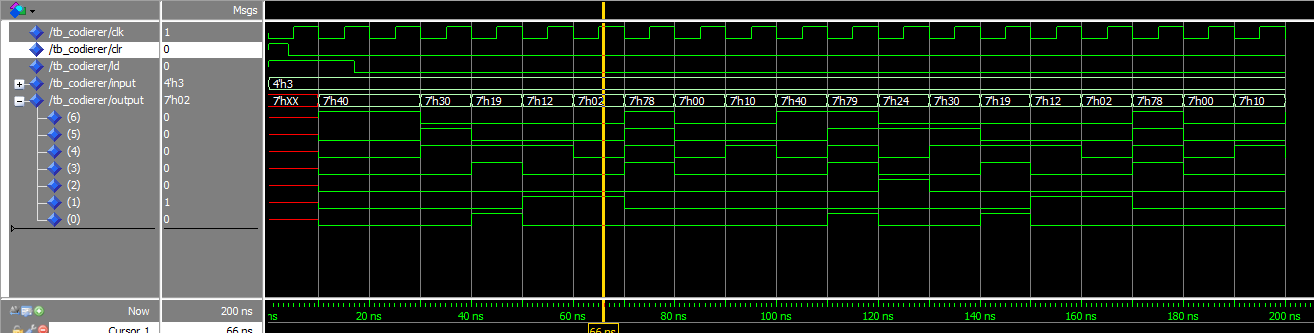
\includegraphics[width=1\textwidth]{./../Electronic_Design_Automation/Lab03_Counters/codierung_simulation.png}}
	\captionof{figure}{Modelsim Simulation}
\end{figure}

\clearpage
\subsection{2-Digit BCD-Arithmetik}

\subsection{3-Digit BCD-Z�hler und 24h-Uhr}

\clearpage
\section{Booth-Algorithmus mit Datenpfad und Steuerwerk}
Das Flu�diagramm nach Abbildung \ref{fig:l4} beschreibt die vorzeichenrichtige Multiplikation von Zahlen im Zweierkomplement durch den sog. Booth-Algorithmus.

Der Multiplikand X wird in das Register M geladen, der Multiplikator Y in das Register P. Das Register A dient als Akkumulator. Das Ergebnis bildet sich im Akkumulator und im Register P.


\begin{figure}[H]
	\centering
	
\includegraphics[width=.8\textwidth,
	page=64,
	trim=3cm 7.5cm 3cm 6.5cm,
	clip]
	{../Labor_PL_Gregorius.pdf}
	\caption{L4 ASM-Chart Booth-Algorithmus}
	\label{fig:l4}
\end{figure}

\clearpage
\subsection{Aufgabenstellungen A}
Anhand des Booth-Algorithmus wird eine Multiplikation (bzw. Division) zweier vorzeichenbehafteten Zahlen in $n$ Schritte durchgef�hrt, wobei $n$ der Anzahl der als Ergebnis darzustellenden Bits entspricht. \\\\
\begin{wrapfigure}{r}{0.4\textwidth}
	\begin{tabular}{c|c}
		\hline
		\noalign{\vskip 3pt}
		Bitkombination & Operation\\
		\noalign{\vskip 3pt}
		\hline
		\noalign{\vskip 3pt}
		01 & Addition \\
		10 & Subtraktion \\
		00 / 11 & - \\
		\hline
	\end{tabular}
\end{wrapfigure}
Dieser Algorithm ist besonders bei einer l�ngeren Rechengr��e geeignet, da die Anzahl partieller Produkte reduziert werden kann.\\\\ 



Im Folgenden werden die handschriftlichen Berechnungen von drei Multiplikationen gezeigt.\\\\

%%
\noindent $P_{1,10} = 2 \cdot 2 \Rightarrow P_{1,2} = 0010 \cdot 0010$\\
$M = 0010$\\

\begin{table}[!h]
	\begin{tabular}{c|c|c|c|c}
		\hline
		\noalign{\vskip 3pt}
		\multirow{2}{*}{}Schritt & A & P Register & Platzhalter & Durchgef�hrte\\
		& & & & Operation\\
		\noalign{\vskip 3pt}
		\hline
		\noalign{\vskip 3pt}
		Init. & 0000 & 0010 & 0 & \\
		\hline
		\multirow{2}{*}{1} & & & & Check Bits: 00\\
		& 0000 & 0001 & 0 & Schift \\
		\hline
		\multirow{3}{*}{2} & & & & Check Bits: 10\\
		& 1110 & 0001 & 0 & $A \leftarrow A-M$\\
		& 1111 & 0000 & 1 & Schift \\
		\hline
		\multirow{3}{*}{3} & & & & Check Bits: 01\\
		& 0001 & 0000 & 1 & $A \leftarrow A+M$\\
		& 0000 & 1000 & 0 & Schift \\
		\hline
		\multirow{2}{*}{4} & & & & Check Bits: 00\\
		& 0000 & 0100 & 0 & Schift \\
		\hline
	\end{tabular}
\end{table}

\noindent Ergebnis: $P_{1,2_{A,P}} = 00000100 \Rightarrow P_{1,10_{A,P}} = 4$\\
%%
\vspace{0.3cm}\\
%%
\noindent $P_{2,10} = 6 \cdot 7 \Rightarrow P_{2,2} = 0110 \cdot 0111$\\
$M = 0110$\\

\begin{table}[!h]
	\begin{tabular}{c|c|c|c|c}
		\hline
		\noalign{\vskip 3pt}
		\multirow{2}{*}{}Schritt & A & P Register & Platzhalter & Durchgef�hrte\\
		& & & & Operation\\
		\noalign{\vskip 3pt}
		\hline
		\noalign{\vskip 3pt}
		Init. & 0000 & 0111 & 0 & \\
		\hline
		\multirow{3}{*}{1} & & & & Check Bits: 10\\
		& 1010 & 0111 & 0 & $A \leftarrow A-M$\\
		& 1101 & 0011 & 1 & Schift \\
		\hline
		\multirow{2}{*}{2} & & & & Check Bits: 11\\
		& 1110 & 1001 & 1 & Schift \\
		\hline
		\multirow{2}{*}{3} & & & & Check Bits: 11\\
		& 1111 & 0100 & 1 & Schift \\
		\hline
		\multirow{3}{*}{4} & & & & Check Bits: 01\\
		& 0101 & 0100 & 1 & $A \leftarrow A+M$\\
		& 0010 & 1010 & 0 & Schift \\
		\hline
	\end{tabular}
\end{table}

\noindent Ergebnis: $P_{2,2_{A,P}} = 00101010 \Rightarrow P_{2,10_{A,P}} = 42$
%%
\vspace{0.3cm}\\
%%
\clearpage
\noindent $P_{3,10} = 6 \cdot (-7) \Rightarrow P_{3,2} = 0110 \cdot 1001$\\
$M = 0110$\\

\begin{table}[!h]
	\begin{tabular}{c|c|c|c|c}
		\hline
		\noalign{\vskip 3pt}
		\multirow{2}{*}{}Schritt & A & P Register & Platzhalter & Durchgef�hrte\\
		& & & & Operation\\
		\noalign{\vskip 3pt}
		\hline
		\noalign{\vskip 3pt}
		Init. & 0000 & 1001 & 0 & \\
		\hline
		\multirow{3}{*}{1} & & & & Check Bits: 10\\
		& 1010 & 1001 & 0 & $A \leftarrow A-M$\\
		& 1101 & 0100 & 1 & Schift \\
		\hline
		\multirow{3}{*}{2} & & & & Check Bits: 01\\
		& 0011 & 0100 & 1 & $A \leftarrow A+M$\\
		& 0001 & 1010 & 0 & Schift \\
		\hline
		\multirow{2}{*}{3} & & & & Check Bits: 00\\
		& 0000 & 1101 & 0 & Schift \\
		\hline
		\multirow{3}{*}{4} & & & & Check Bits: 10\\
		& 1010 & 1101 & 0 & $A \leftarrow A-M$\\
		& 1101 & 0110 & 1 & Schift \\
		\hline
	\end{tabular}
\end{table}

\noindent Ergebnis: $P_{3,2_{A,P}} = 11010110 \Rightarrow P_{3,10_{A,P}} = -42$
%%

\subsubsection{Arithmetische Einheit}
\label{chap:L4_B1}
Abbildung \ref{fig:l4B1} zeigt eine aus Datenpfad und Steuerwerk bestehende arithmetische Einheit, die das Produkt von zwei 4-Bit Zweirkomplement-Zahlen nach dem Booth-Algorithmus berechnet.

\begin{figure}[H]
	\centering
	%<<<<<<< HEAD
	%	\includegraphics[width=.7\textwidth]{421}
	%	\caption{L4 Arithmetische Einheit}
	%=======
	\includegraphics[width=.8\textwidth,
	page=2,
	trim=4.2cm 4.5cm 4.2cm 18.6cm,
	clip]
	{muster06.pdf}
	\caption{L4 Arithmetische Einheit f�r den Booth-Algorithmus}
	%>>>>>>> 8043616c7aa25e52d88a3ff2d89b4efbde4f8389
	\label{fig:l4B1}
\end{figure}

Die Funktionalit�t der Arithmetischen Einheit, bereits um INBUS und OUTBUS erweitert, ist wie Folgt:

\begin{tabular}{r l}
	\small{Bezeichnung} & \small{Beschreibung} \\ 
	Reset & Zur�cksetzung in den Anfangszustand (alle Registerinhalte auf Null) \\
	LM    & �bernahme der Daten aus dem INBUS in das M-Register \\
	LQ    & �bernahme der Daten aus dem INBUS in das Q-Register \\
	Add   & Addition von M und A, die Summe wird in A geschrieben \\
	Sub   & Subtraktion von M und A, die Differenz wird in A geschrieben \\
	Shift & A und Q werden gemeinsam nach rechts geschoben, Bit 0 wird dupliziert \\
	Inc   & Der Z�hler wird um eins erh�ht \\
	StA   & Der Inhalt von A wird an den OUTBUS �bergeben \\
	StQ   & Der Inhalt von Q wird an den OUTBUS �bergeben \\
	E3    & Der Z�hler ist gleich drei \\
	x1    & Bit n-1 aus Q \\
	x0    & Bit n aus Q \\
\end{tabular}

\subsubsection{Moore-Automaten}
Abbildung \ref{fig:l4b4} zeigt einen dem Flussdiagramm (Abb. \ref{fig:l4}) entsprechenden Moore-Automaten.
%\afterpage{%
\begin{figure}[H]
	\centering
	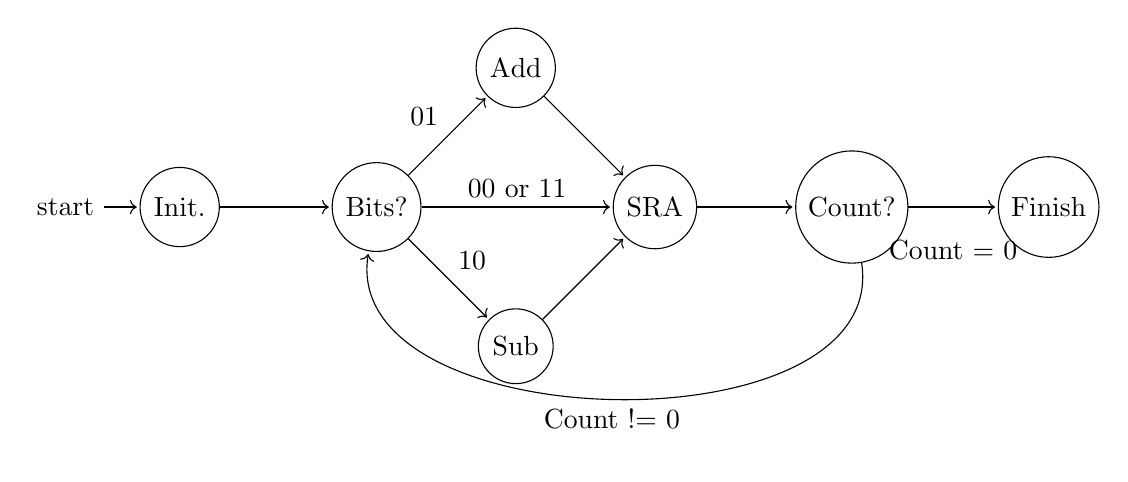
\begin{tikzpicture}[shorten >=1pt,node distance=2.5cm,on grid,auto] 
	\node[state,initial] (init) {Init.};
	\node[state] (checkB) [right=of init] {Bits?};  
	\node[state] (add) [above right=of checkB] {Add};
	\node[state] (sub) [below right=of checkB] {Sub};
	\node[state] (shift) [below right=of add] {SRA};
	\node[state] (checkC) [ right=of shift] {Count?};
	\node[state] (f) [ right=of checkC] {Finish};
	\path[->]
	(init) edge node {} (checkB)
	(checkB) edge node {01} (add)
	(checkB) edge node {10} (sub)
	(checkB) edge node {00 or 11} (shift)
	(add) edge node {} (shift)
	(sub) edge node {} (shift)
	(shift) edge node {} (checkC)
	(checkC) edge [bend left=100] node {Count != 0} (checkB)
	(checkC) edge node [below=0.3] {Count = 0} (f)
	;
	\end{tikzpicture}
	\caption{Moore-Automaten}\label{fig:l4b4}
\end{figure}
%}%

\subsubsection{VHDL Beschreibung}

\begin{figure}[!hb]
	\centering
	\fbox{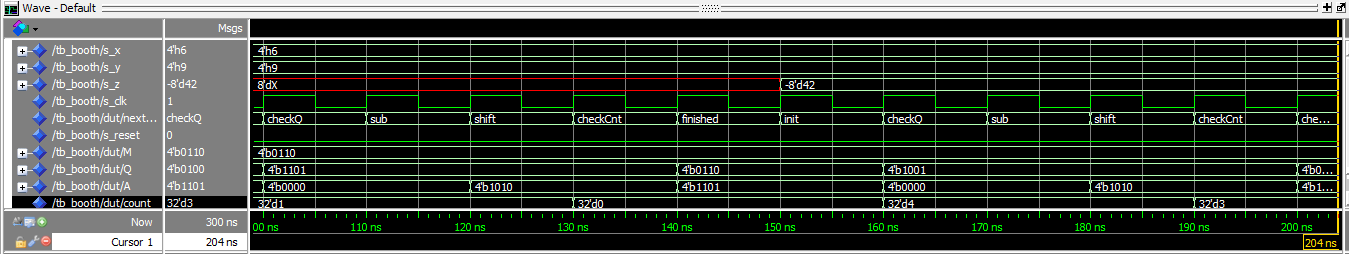
\includegraphics[width=1\textwidth]{./../Electronic_Design_Automation/Lab04_Booth_Algorithm/booth_simulation.png}}
	\captionof{figure}{State Machine Modelsim Simulation}
\end{figure}

\lstinputlisting[caption=Booth Algorithm VHDL Code]{./../Electronic_Design_Automation/Lab04_Booth_Algorithm/booth.vhd}

\lstinputlisting[caption=Booth Algorithm Testbench]{./../Electronic_Design_Automation/Lab04_Booth_Algorithm/tb_booth.vhd}



\end{document}

